\begin{center}
    \section*{\fontsize{20}{20}\selectfont Chapter 3}
\end{center}
\vspace{10mm}
\section{Proposed Model and Implementation }
\subsection{Introduction}
The development of  Typing Speed Tester project involves a multifaceted exploration, covering various critical aspects essential for its successful execution. This chapter embarks on a comprehensive journey through the project's Feasibility Analysis, Requirement Analysis, The Project Methodology, Data Set details, Data Collection and Preprocessing, Feature Selection, Algorithmic intricacies, and the Design and Implementation considerations.\\

\textbf{ Project Code:}

\begin{figure}[h]
     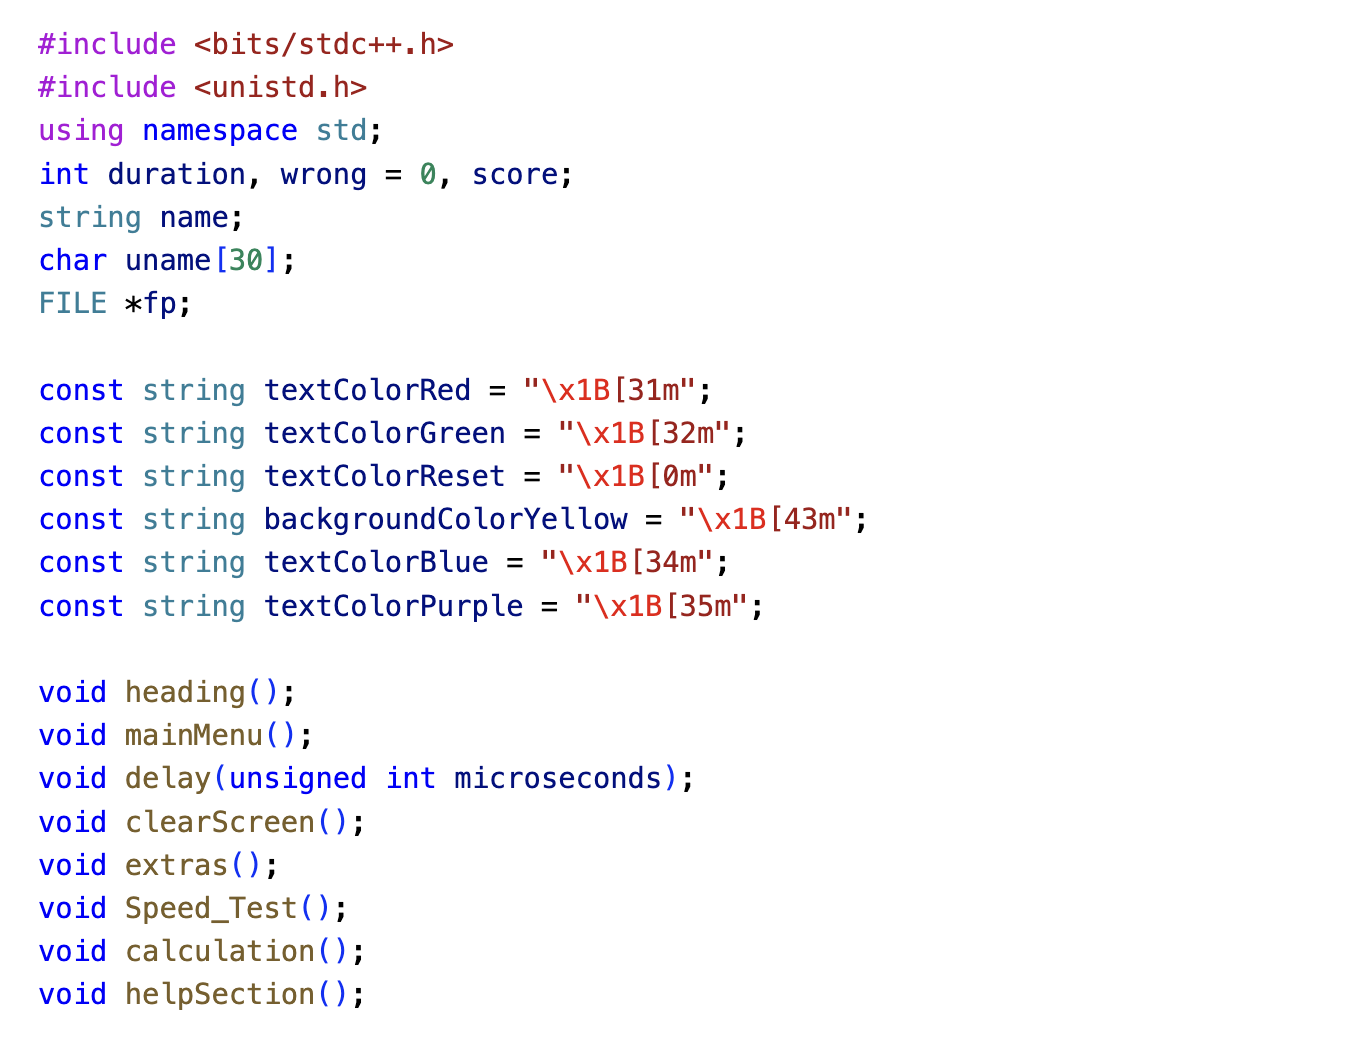
\includegraphics[scale=0.2]{CodeScreenShot/include.png}
    \caption{Code}
    \label{fig:code-screenshots}
\end{figure}

\subsection{Programme Description}

\begin{itemize}

        \item The figure 3.1 shows a text-based console application that offers a series of features to users, including  Speed test,Help,User record information.
\end{itemize}
\newpage
\begin{figure}[h]
     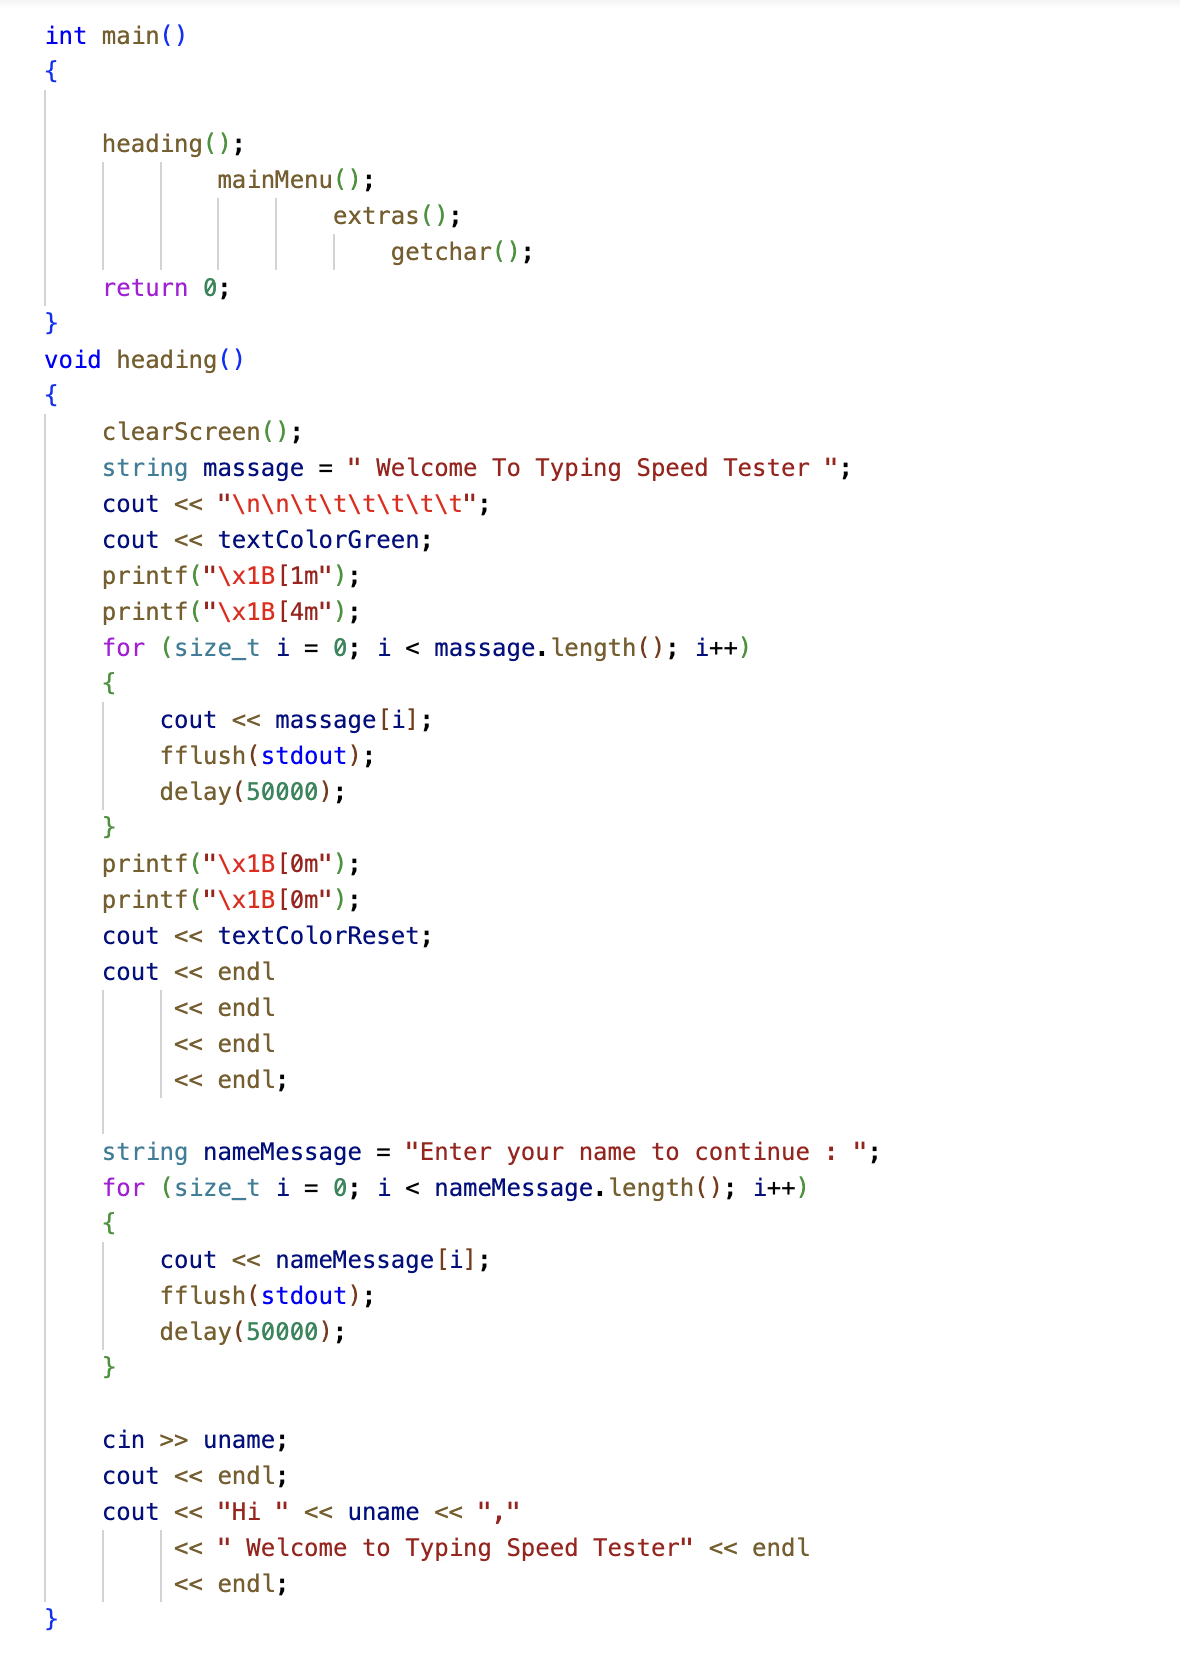
\includegraphics[scale=0.25]{CodeScreenShot/mainAndHeading.png}
    \caption{Code}
    \label{fig:code-screenshots}
\end{figure}

\subsection{Programme Description}

\begin{itemize}

        \item \texttt{ }The main function consist of following functions - heading(),mainMenu(),extras(). This sets the stage for the main menu, presented by the mainMenu function, where users get to choose their typing speed, view records, or access help. The extras function provides additional information, and the program waits for user input before concluding.
    \end{itemize}
\newpage
\begin{figure}[h]
     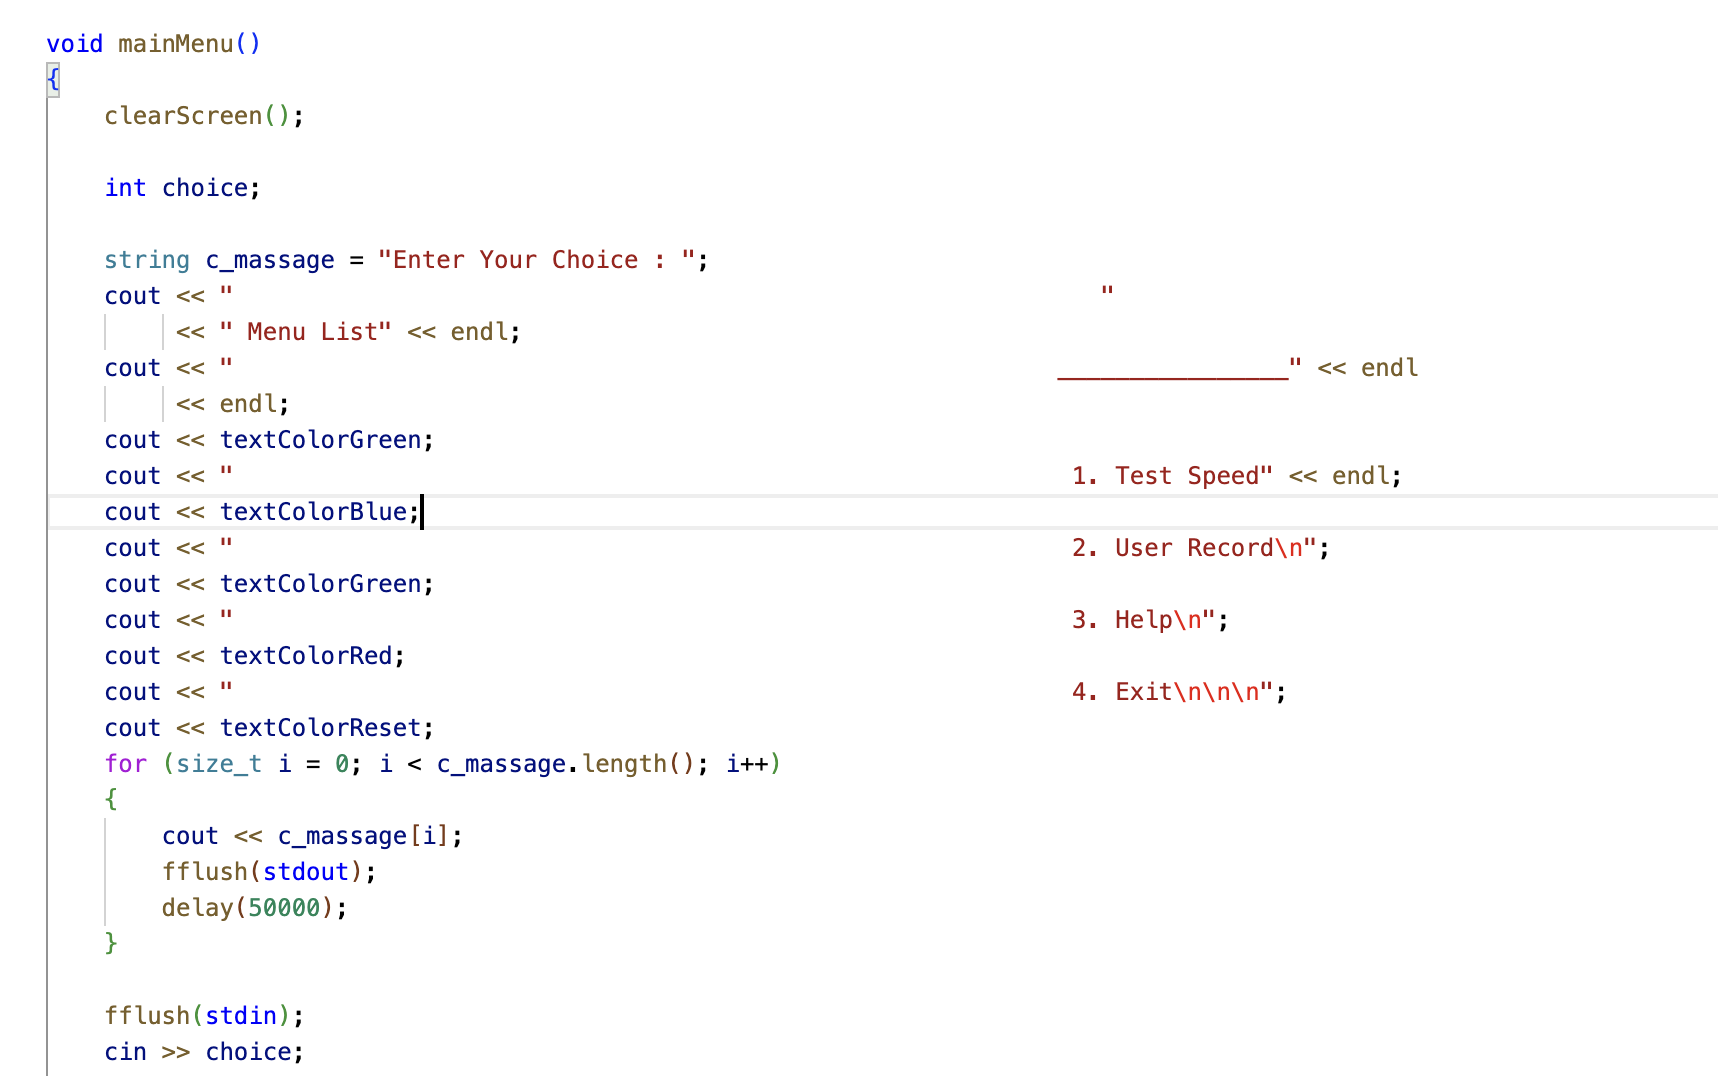
\includegraphics[scale=0.25]{CodeScreenShot/CleanShot 2023-12-05 at 09.19.29@2x.png}
    \caption{Code}
    \label{fig:code-screenshots}
\end{figure}

\subsection{Programme Description}

\begin{itemize}

        \item The mainMenu function presents a user-friendly menu interface, clearing the screen and displaying options for the Typing Speed Tester application. Users are prompted to enter their choice from the menu, including options to test typing speed, view user records, access help, or exit the program. The function incorporates color-coded text for clarity and utilizes a delay effect for a smoother visual presentation.

\end{itemize}
\newpage
\begin{figure}[h]
     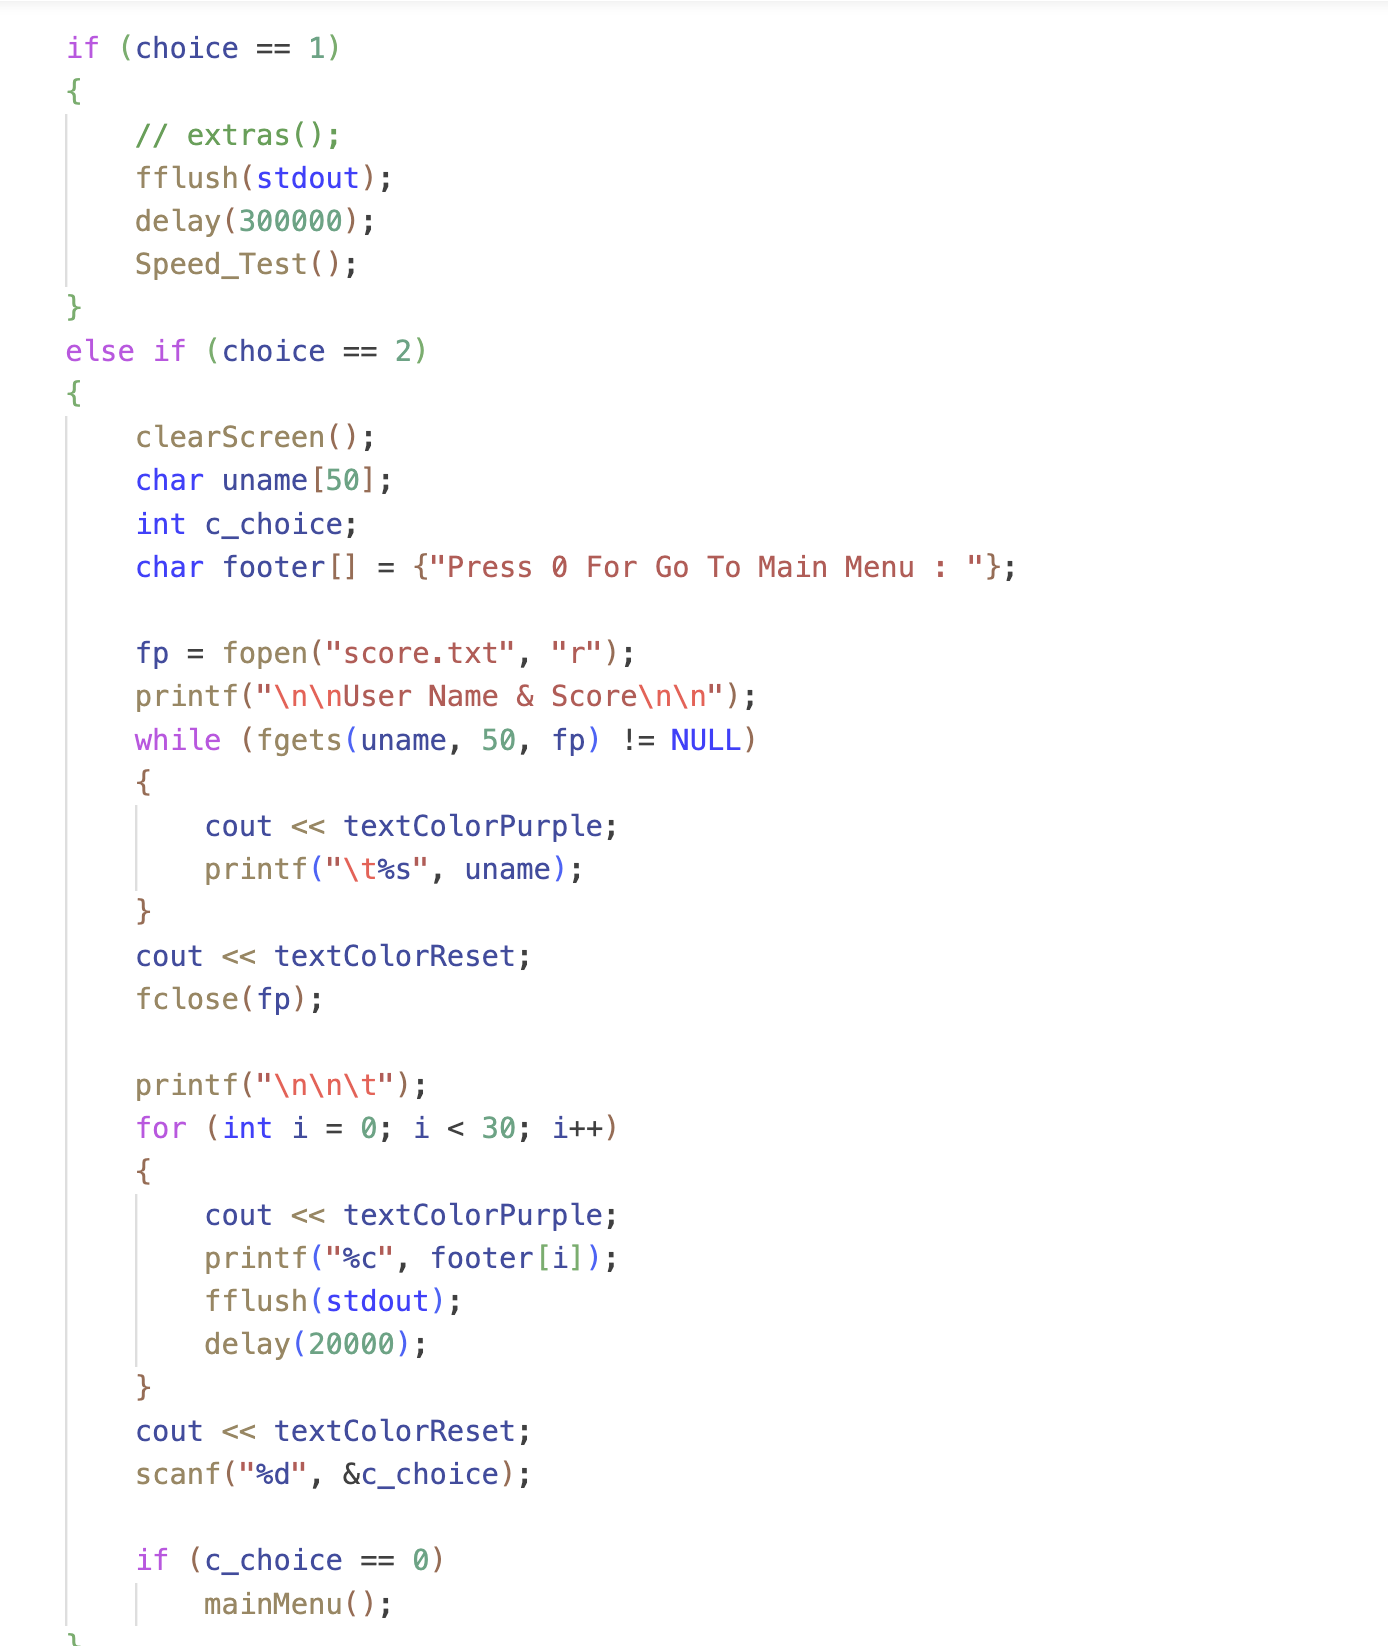
\includegraphics[scale=0.25]{CodeScreenShot/choice1-2.png}
    \caption{Code}
    \label{fig:code-screenshots}
\end{figure}

\subsection{Programme Description}

\begin{itemize}

        \item in this section, if the user's choice is 1, the program initiates a delay before proceeding to the Speed\_Test function, likely for a visual effect or to simulate a pause. If the choice is 2, the program displays a user record section by reading data from a file ("score.txt") and presenting it on the screen. Users are prompted to return to the main menu by entering '0', triggering the mainMenu function. The use of color-coded text enhances the visual appeal of the displayed information.

\end{itemize}
\newpage
\begin{figure}[h]
     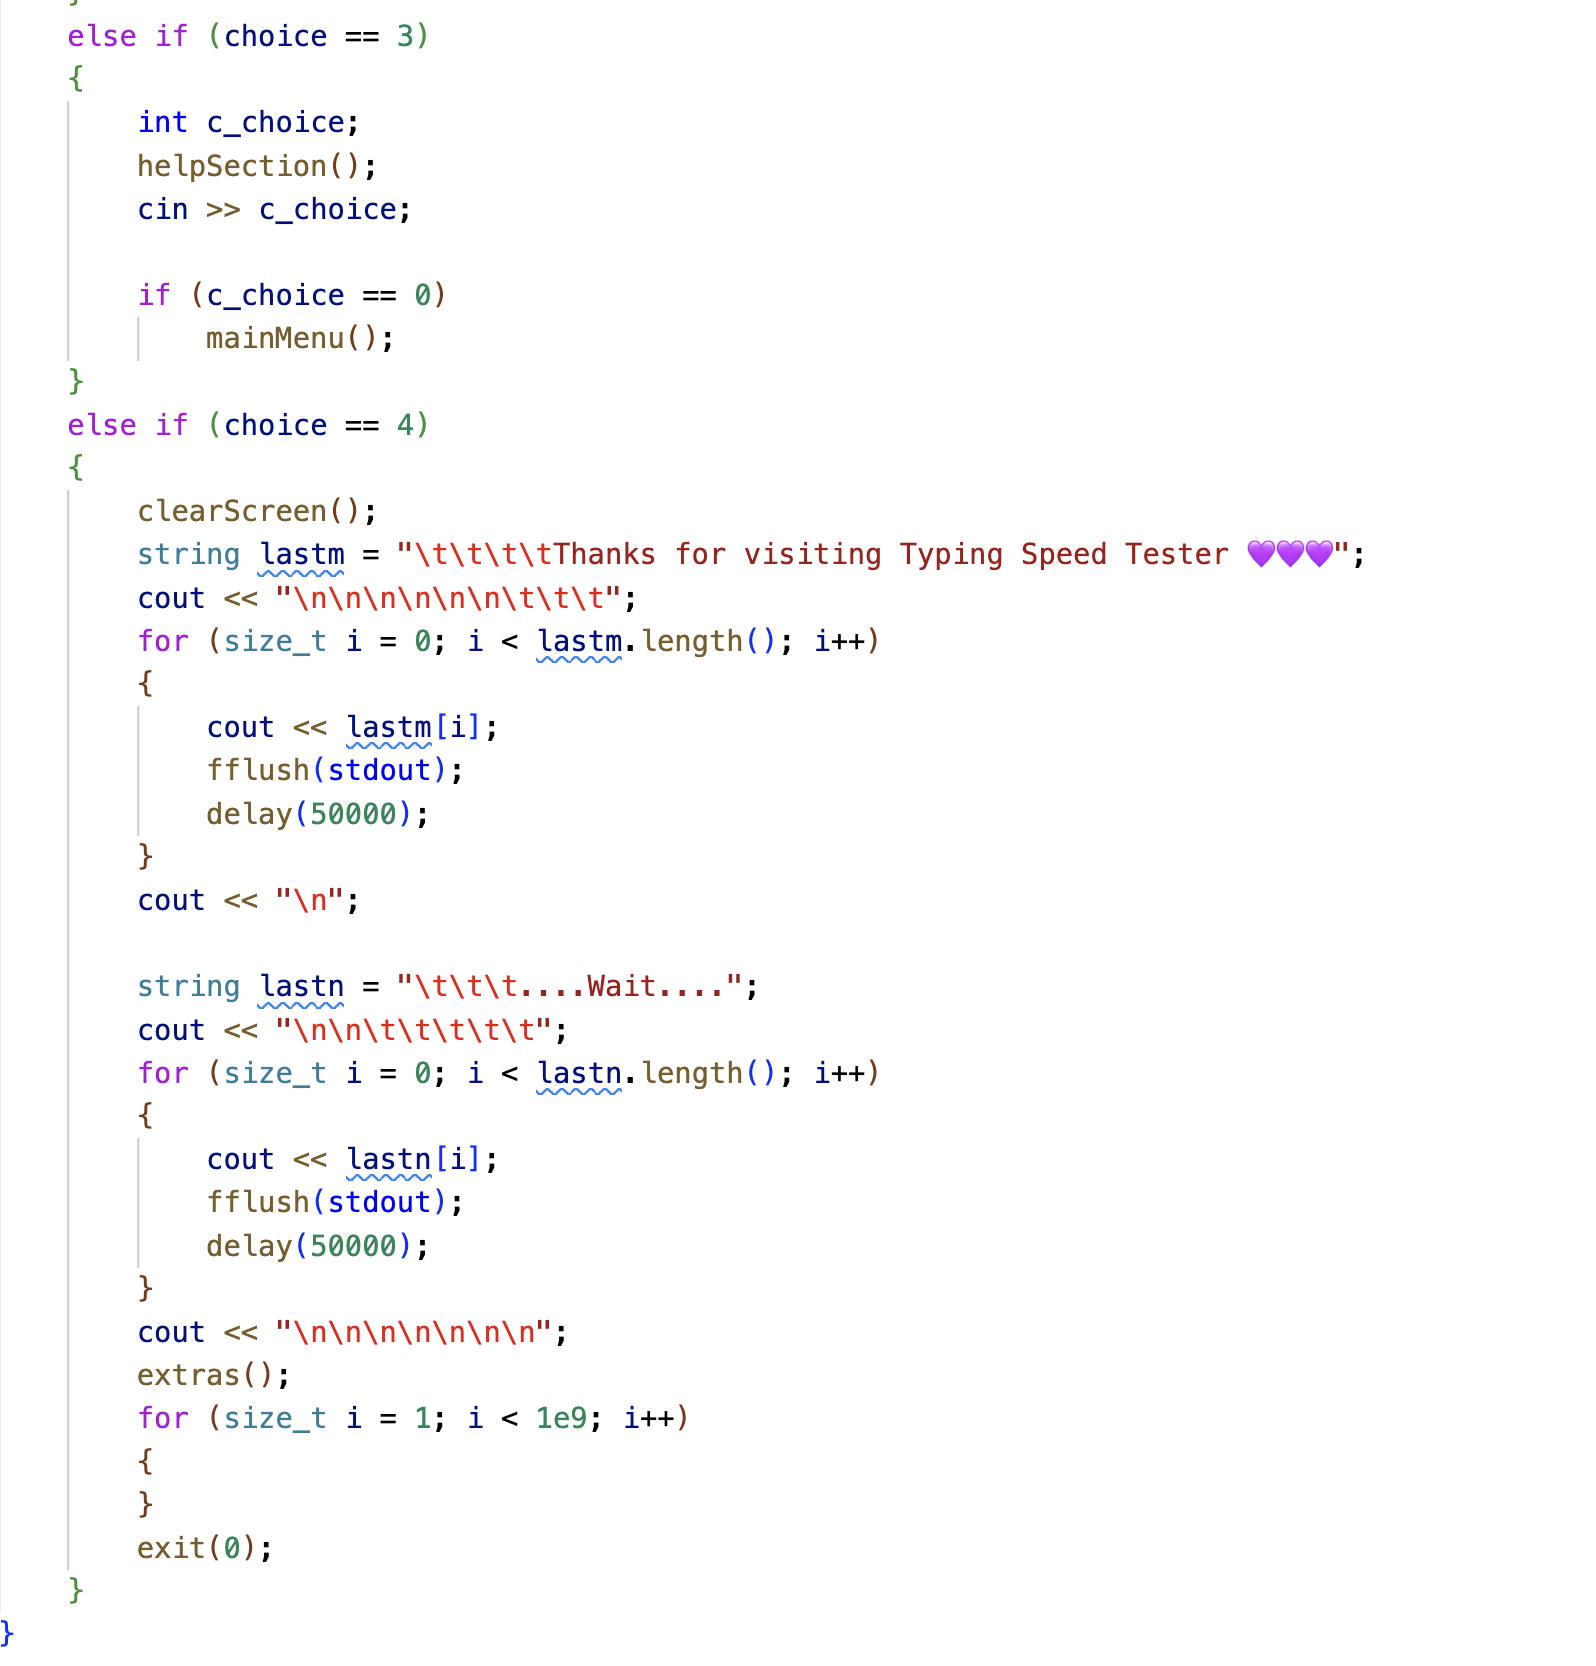
\includegraphics[scale=0.25]{CodeScreenShot/choice3-4.png}
    \caption{Code}
    \label{fig:code-screenshots}
\end{figure}

\subsection{Programme Description}

\begin{itemize}
        \item In this code segment 3.5 corresponds to the handling of menu choice 3 and 4. If the user chooses option 3, it invokes the helpSection() function, likely displaying information or instructions. The user is prompted to enter a choice, and if it's 0, the program returns to the main menu. If the choice is 4, the program displays a farewell message, initiates a brief waiting period, and then exits the program after executing some additional functions in the extras() section. The exit is delayed for a noticeable period, providing a closing effect before terminating the program.
\end{itemize}
\newpage
\begin{figure}[h]
     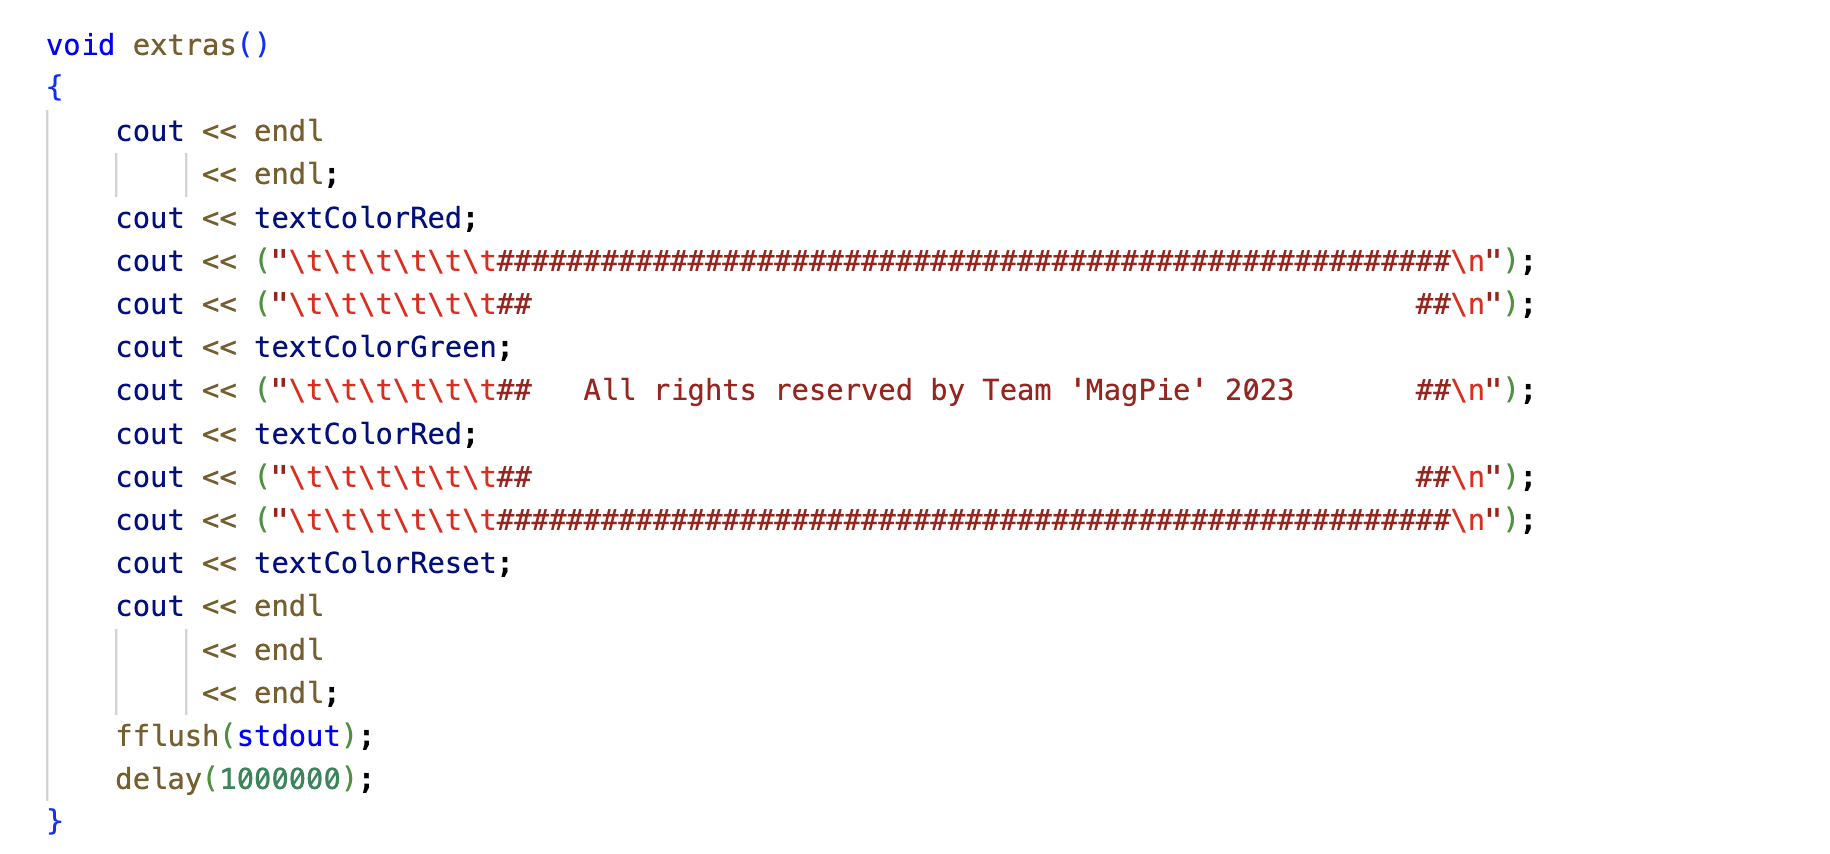
\includegraphics[scale=0.25]{CodeScreenShot/Extra-FooterSection.png}
    \caption{Code}
    \label{fig:code-screenshots}
\end{figure}

% \subsection{The project project allows participants to measure and potentially improve their typing skills.In this figure to enhance the user experience, the tester can be integrated with adjustable font size, text passage selection, audio feedback, and detailed statistics. This interactive approach aims to provide an engaging platform for users to assess and enhance their typing abilities. The project ultimately seeks to facilitate the learning process and create a more personalized and effective typing experience.}
\subsection{Programmme Description}

\begin{itemize}
    \item \textbf{All headers:}
    \begin{itemize}
        \item
        The figure 3.6 captures the extra function which provides the information of the Typing Speed Tester developer team follows the copyright law and all rights are reserved by  team MagPie.
    \end{itemize}
\end{itemize}
\newpage
\begin{figure}[h]
     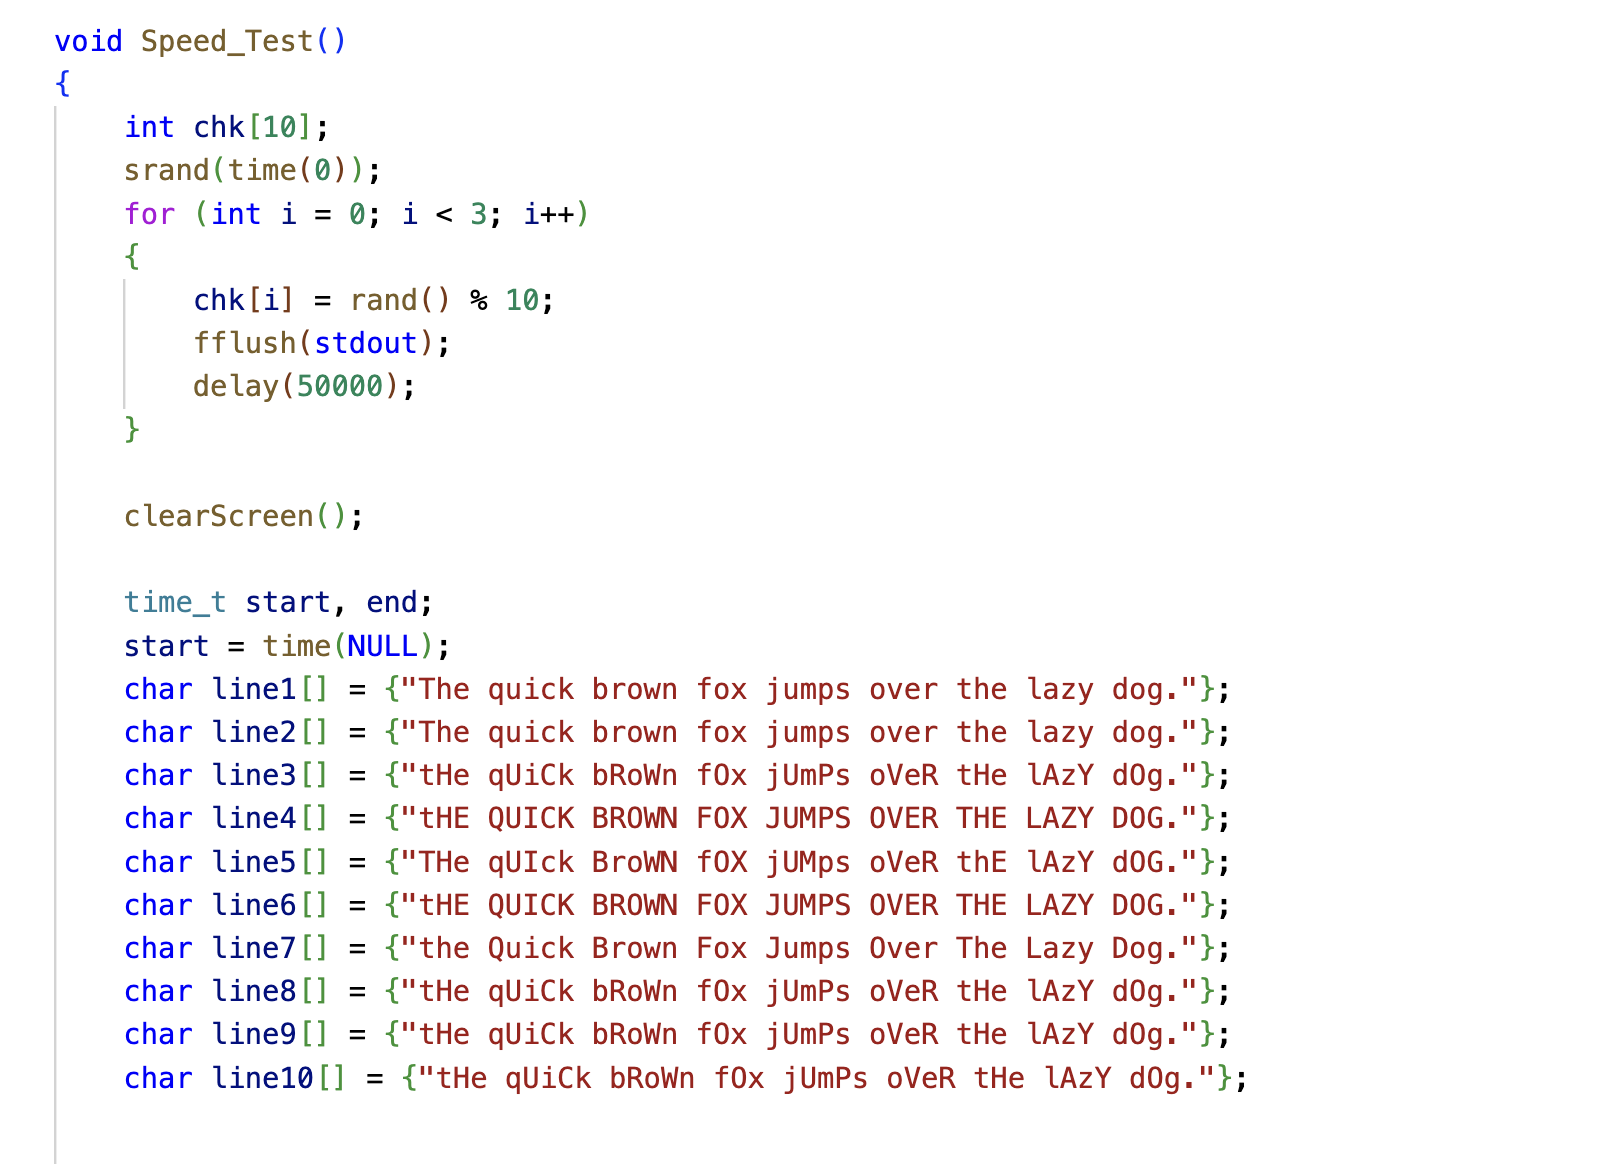
\includegraphics[scale=0.25]{CodeScreenShot/speedtest-1.png}
    \caption{Code}
    \label{fig:code-screenshots}
\end{figure}

\subsection{Programme Description}

    \begin{itemize}
        \item The Speed\_Test function generates a random sequence of indices in the range [0, 9] and stores them in the array chk. It then clears the screen and initializes a timer. The function presents ten different lines of text with variations in letter casing, simulating a typing speed test. The user is likely required to replicate the provided sentences accurately within a time limit, evaluating their typing speed and accuracy. The inclusion of randomization enhances the test's variability, making it more challenging for the user.
    \end{itemize}
\newpage

\begin{figure}[h]
     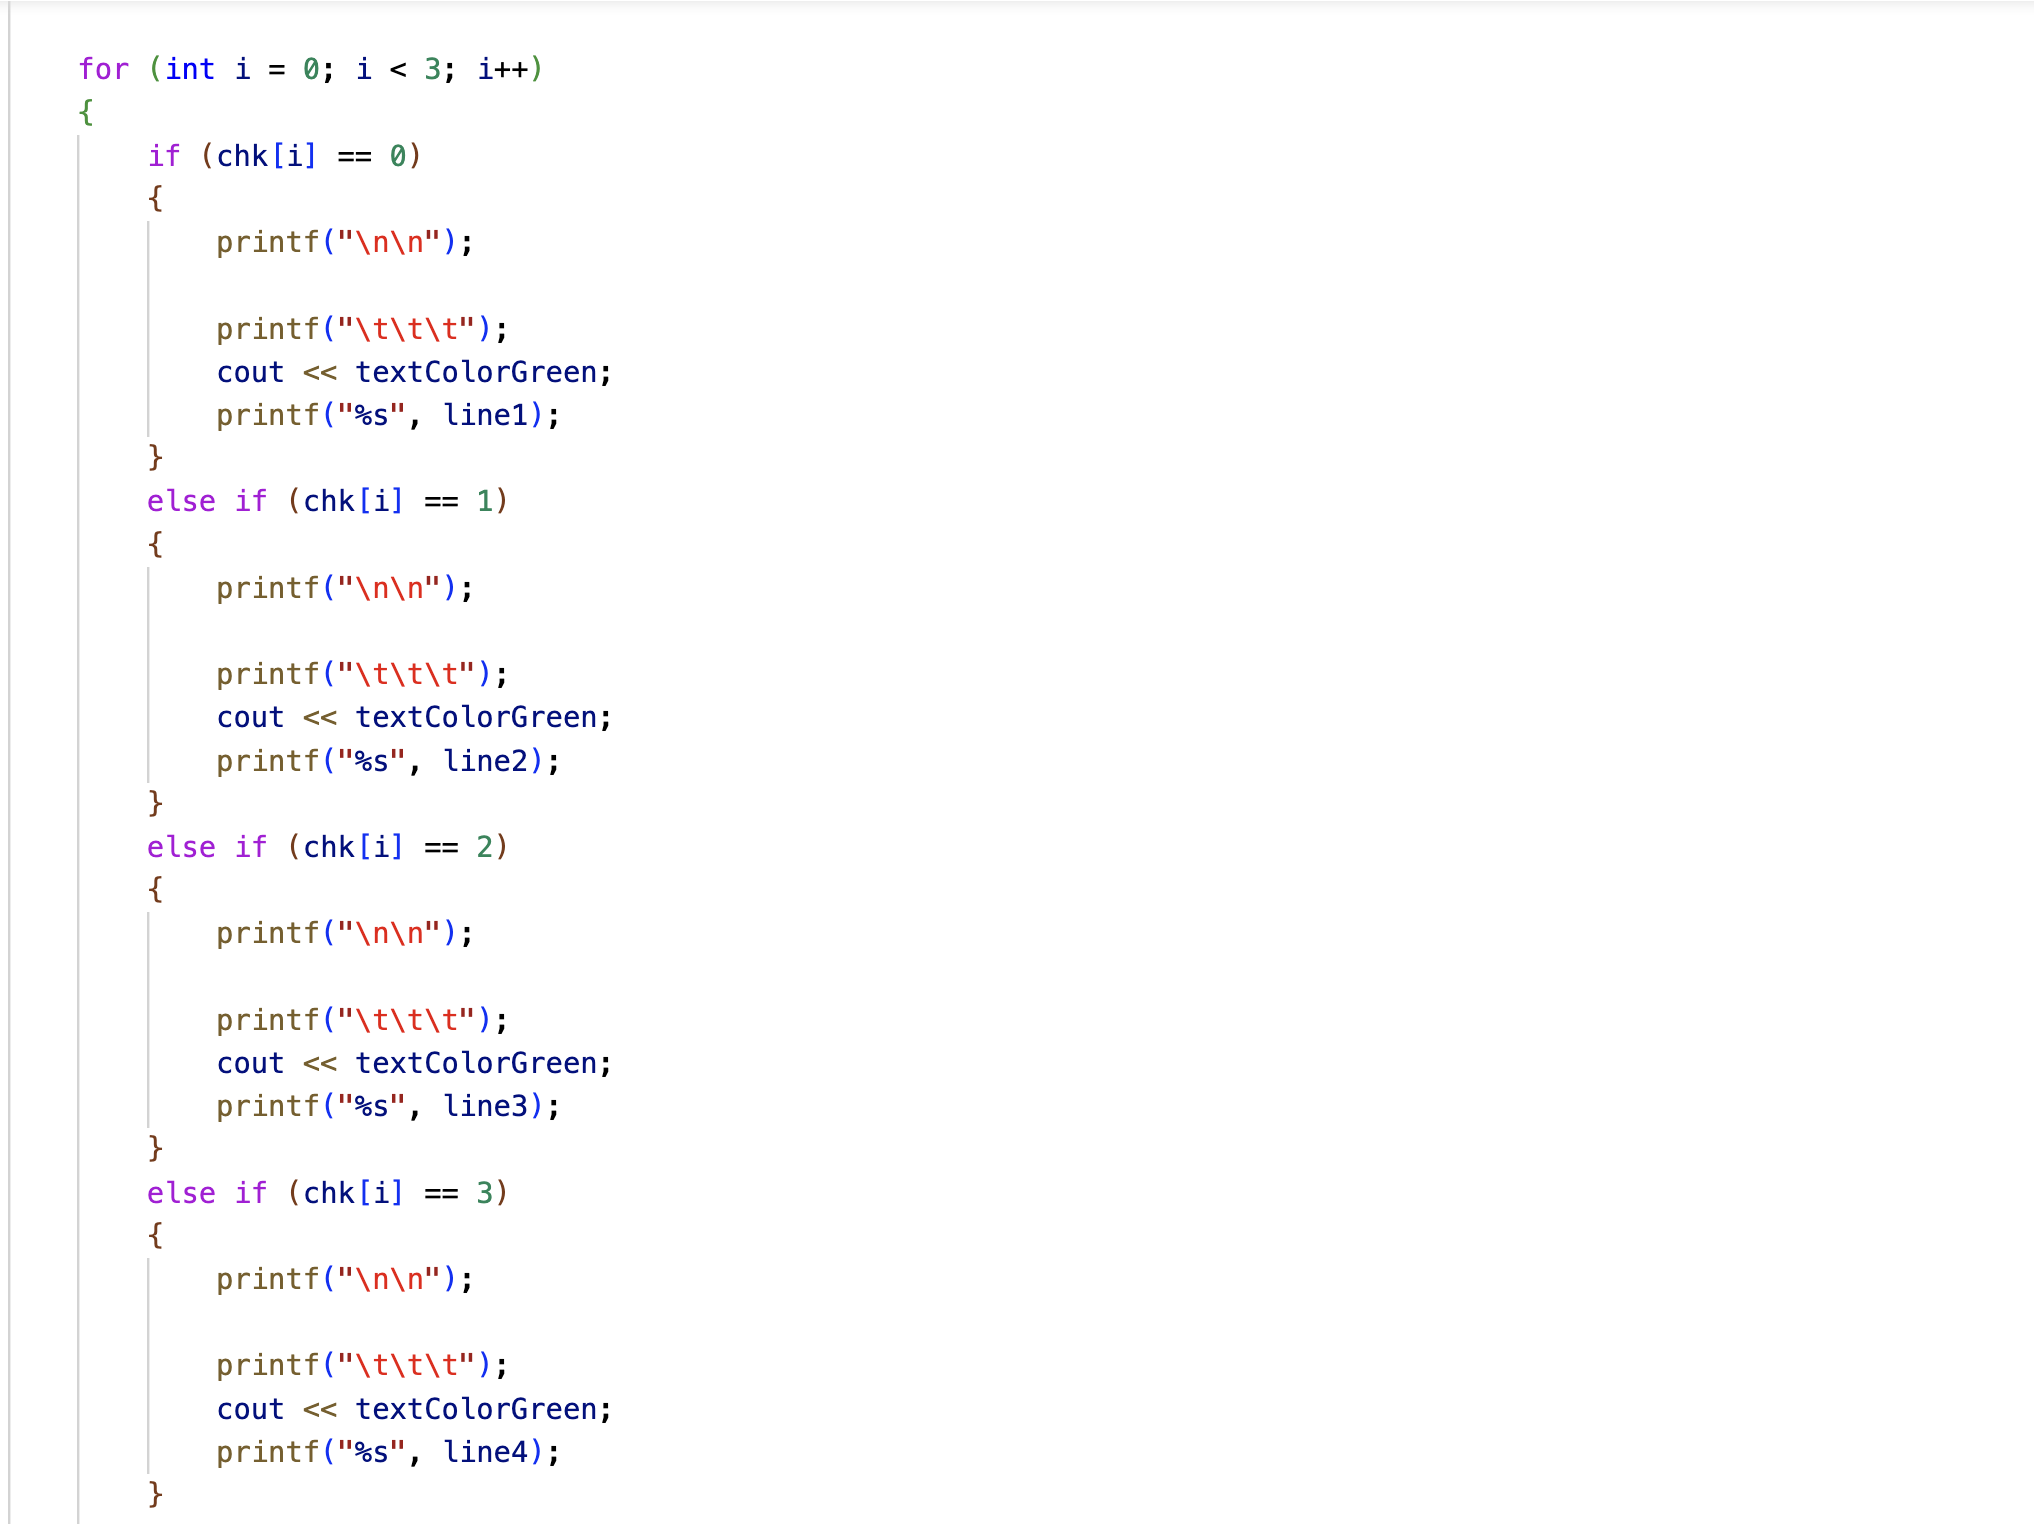
\includegraphics[scale=0.16]{CodeScreenShot/speedtest-2.png}
     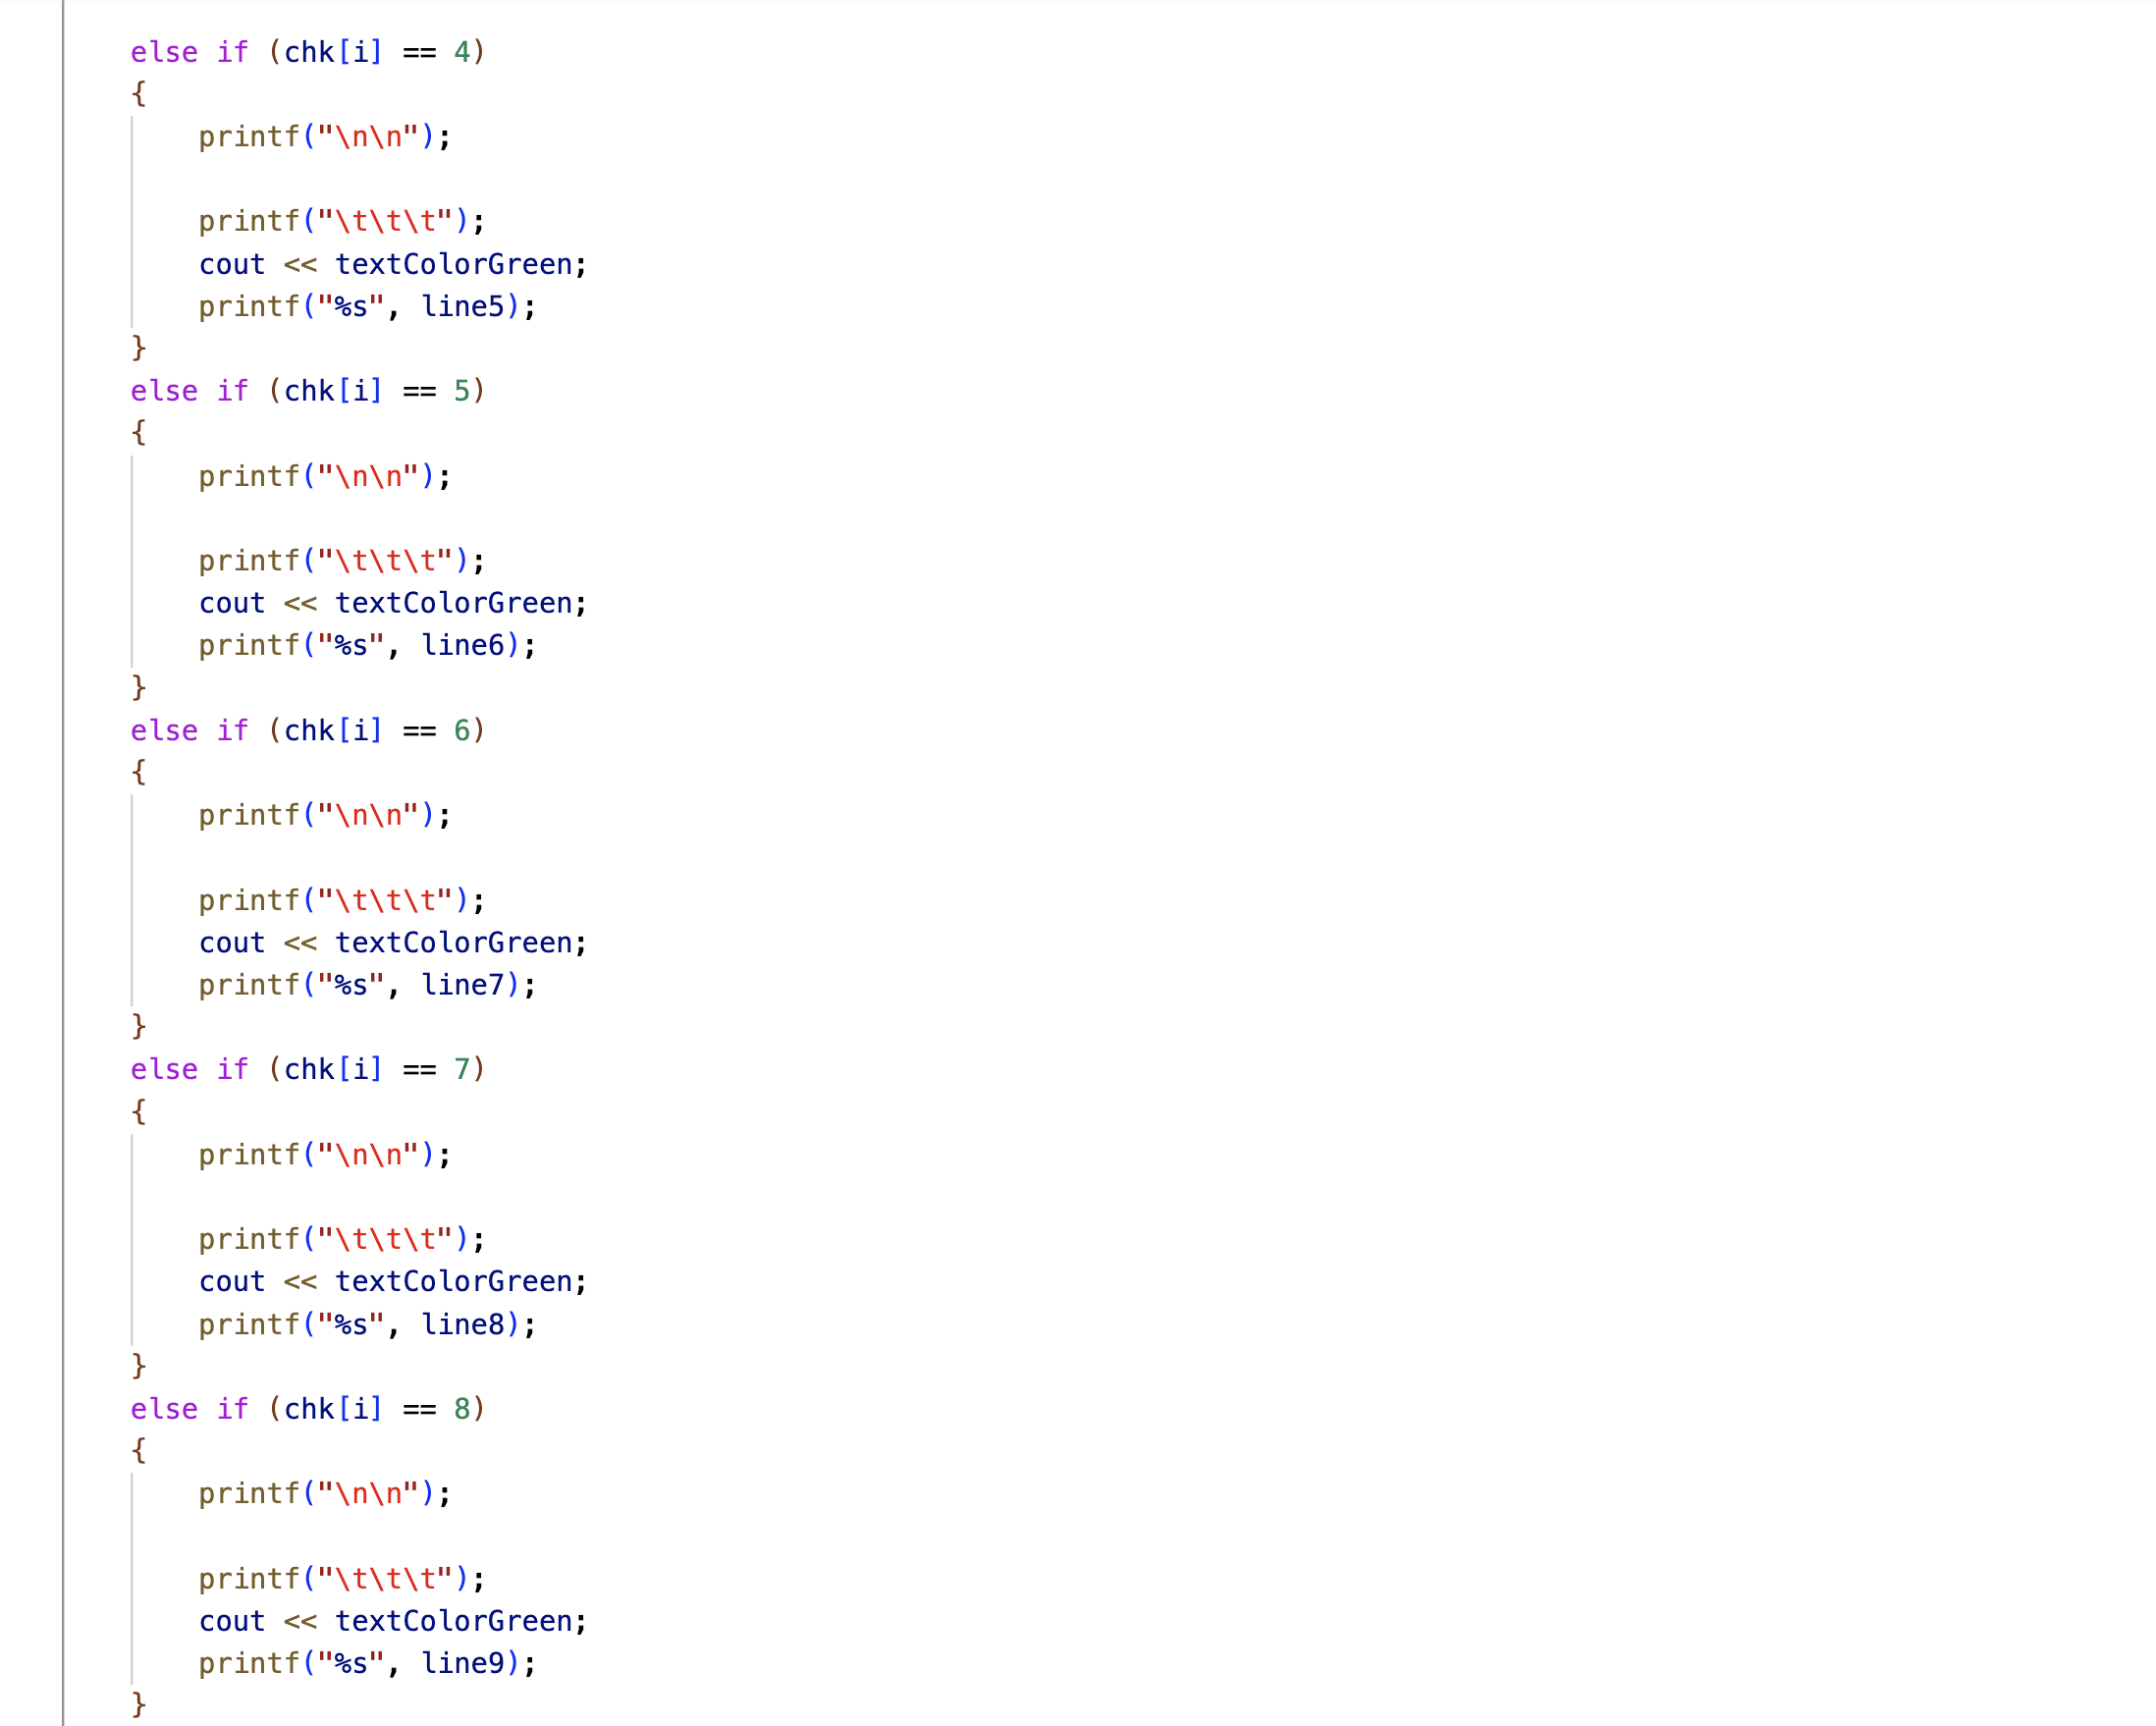
\includegraphics[scale=0.16]{CodeScreenShot/speedtest-3.png}
    \caption{Code}
    \label{fig:code-screenshots}
\end{figure}
\begin{figure}[h]
     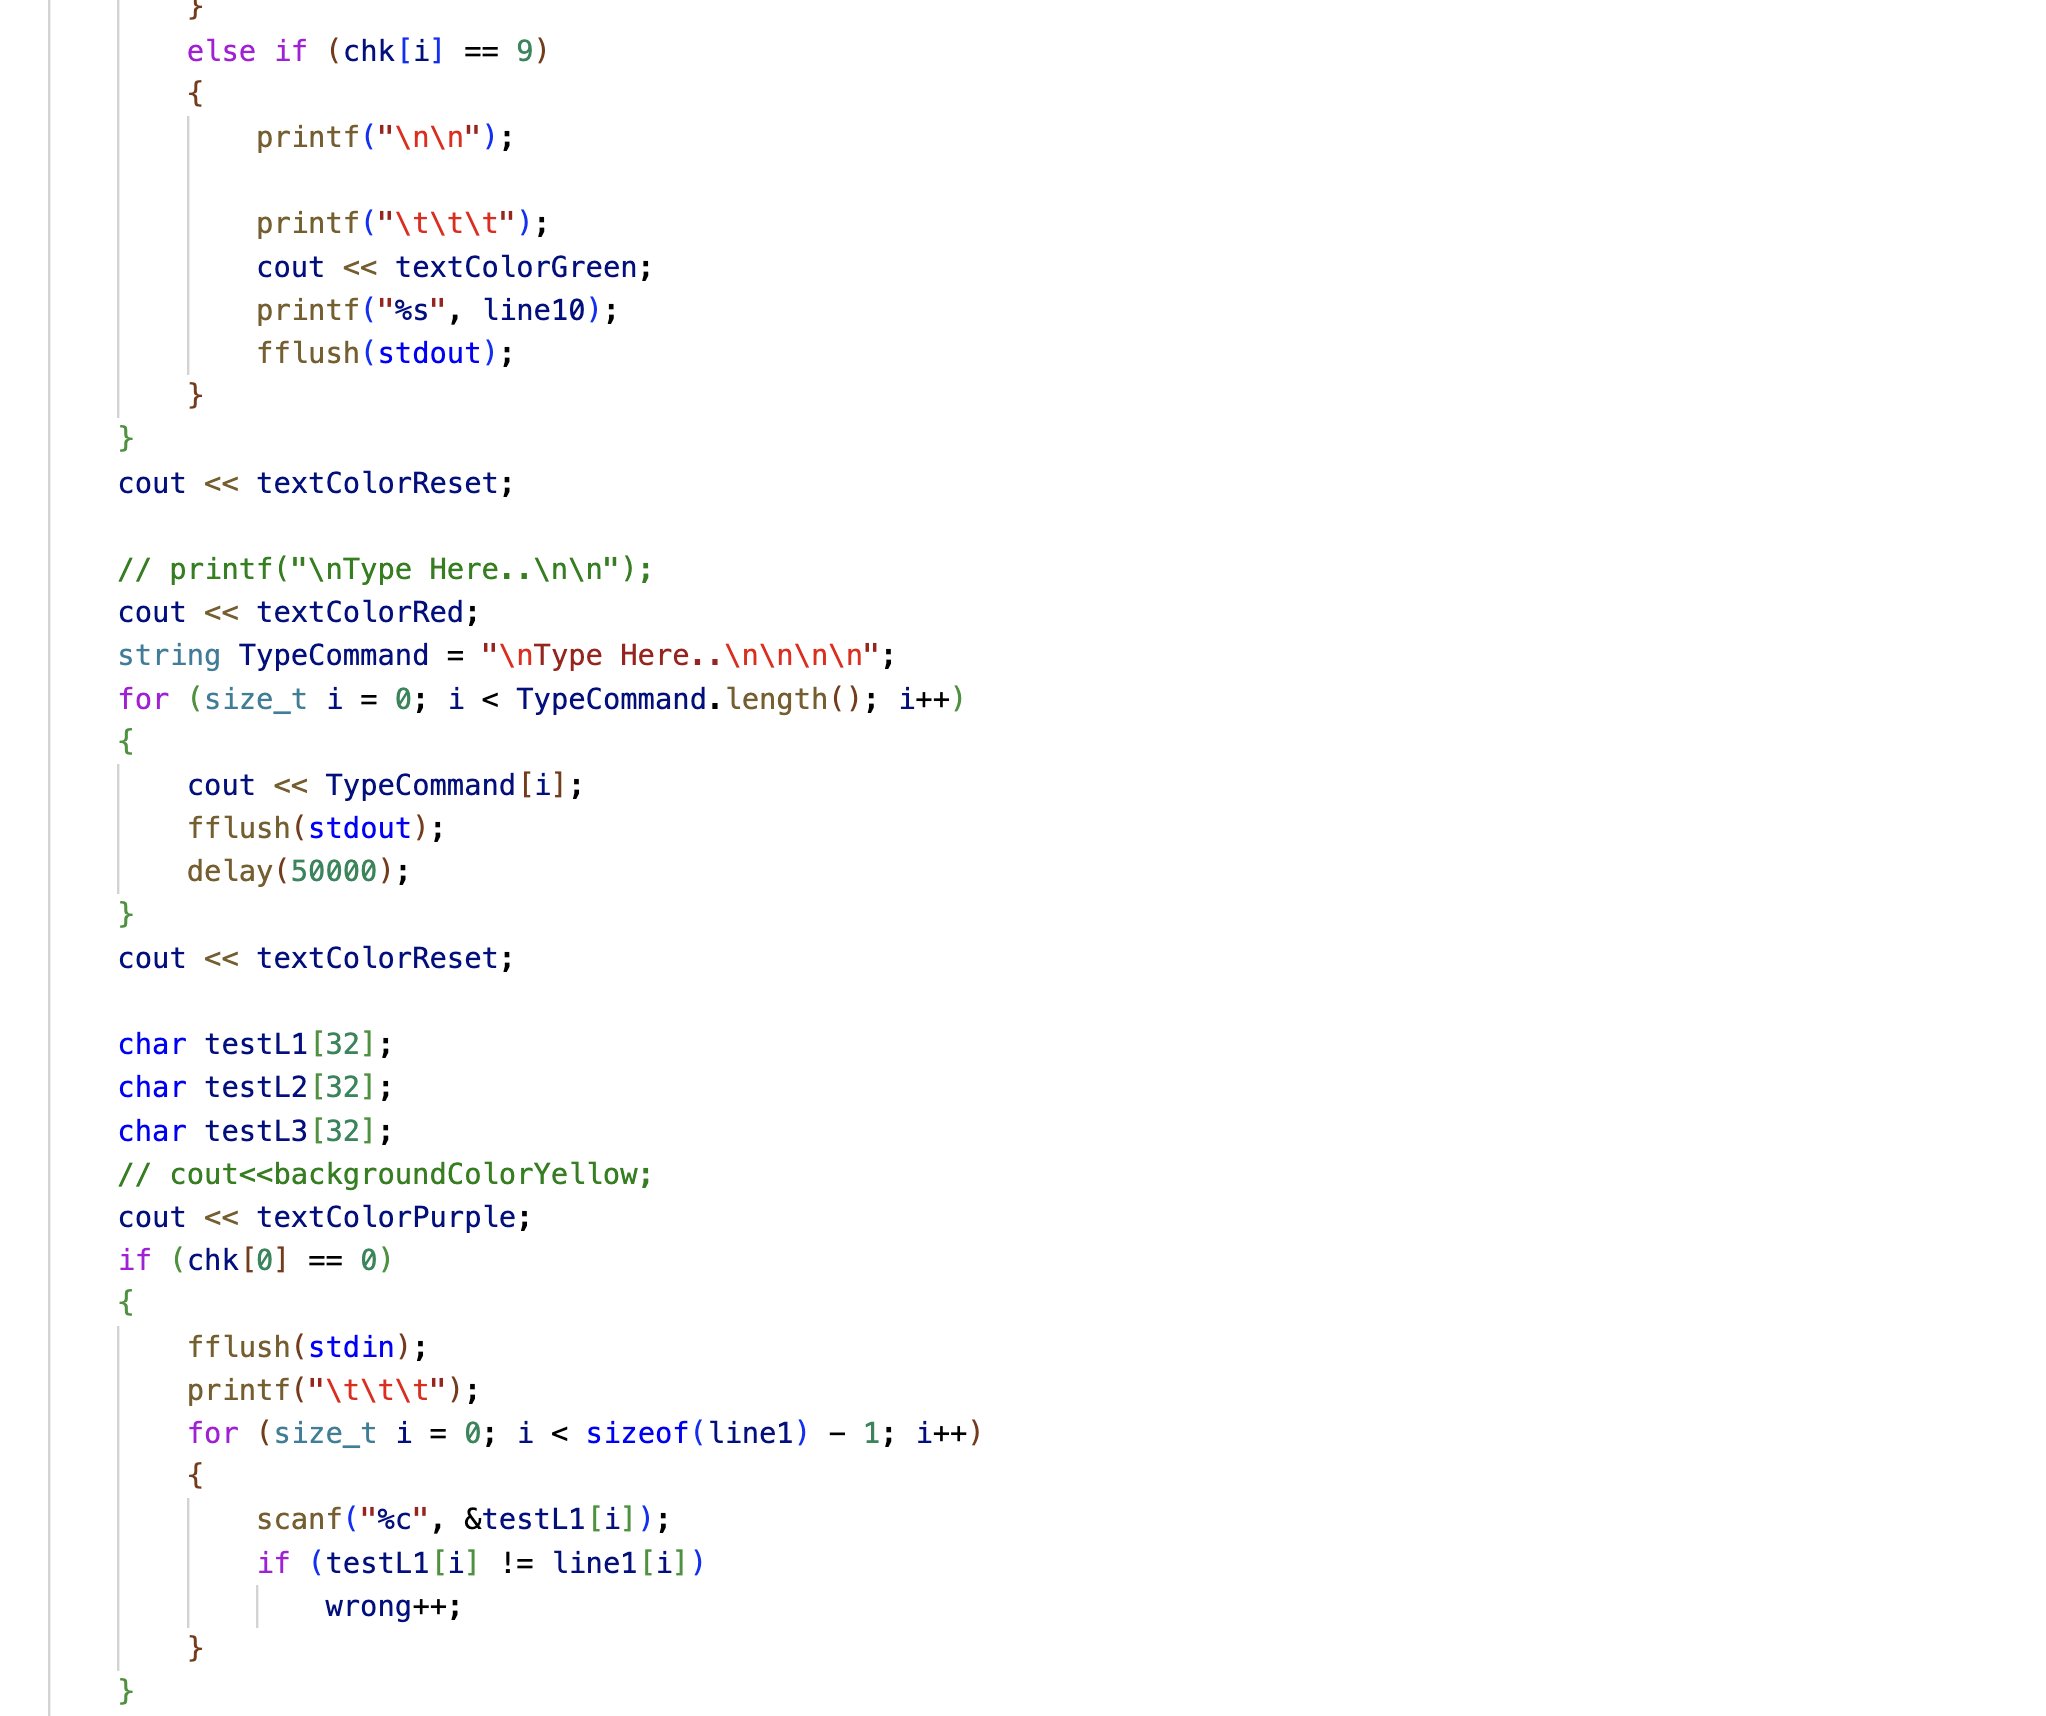
\includegraphics[scale=0.12]{CodeScreenShot/speedtest-4.png}
    \caption{Code}
    \label{fig:code-screenshots}
\end{figure}
\subsection{Programme Description}
    \begin{itemize}
        \item This portion of the code presents three lines randomly selected from a set of predefined text lines (line1 to line10) to the user. The user is then prompted with a "Type Here" command, and their input for the first line is compared character by character. Any discrepancies are tracked, contributing to the 'wrong' counter that monitors input accuracy. Additionally, visual effects using different text colors are applied to enhance the user interface.
    \end{itemize}
\newpage
\begin{figure}[h]
     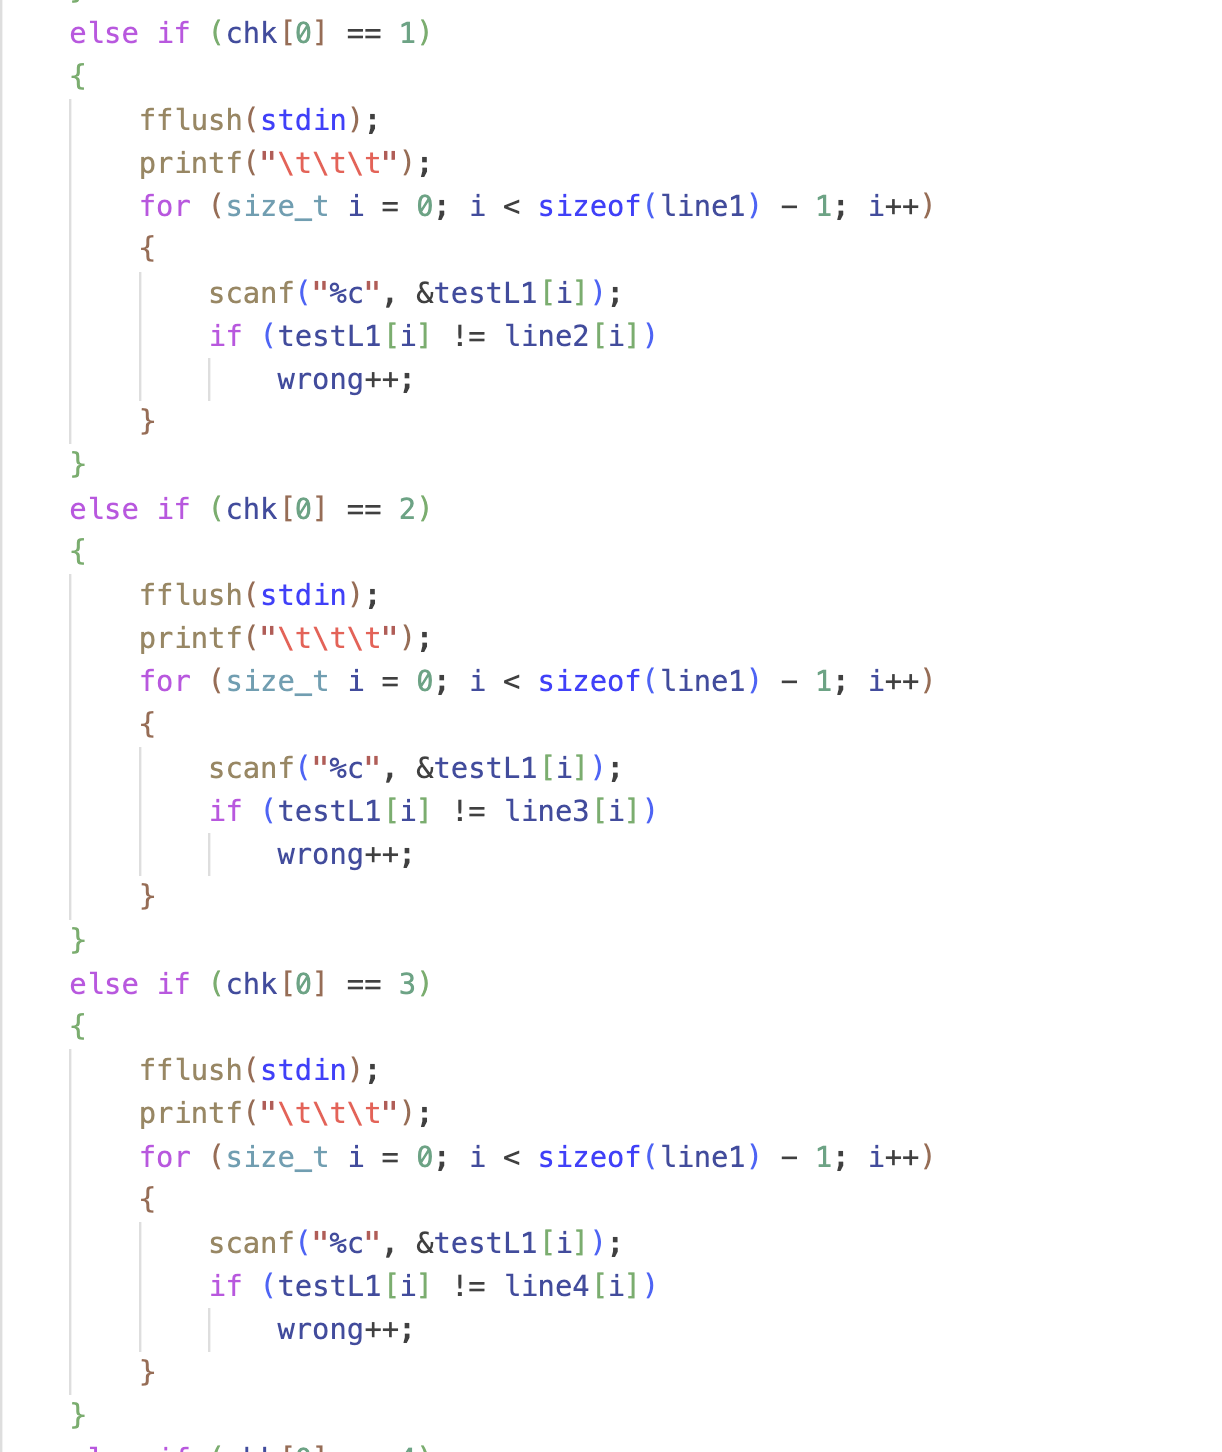
\includegraphics[scale=0.16]{CodeScreenShot/speedtest-6.png}
     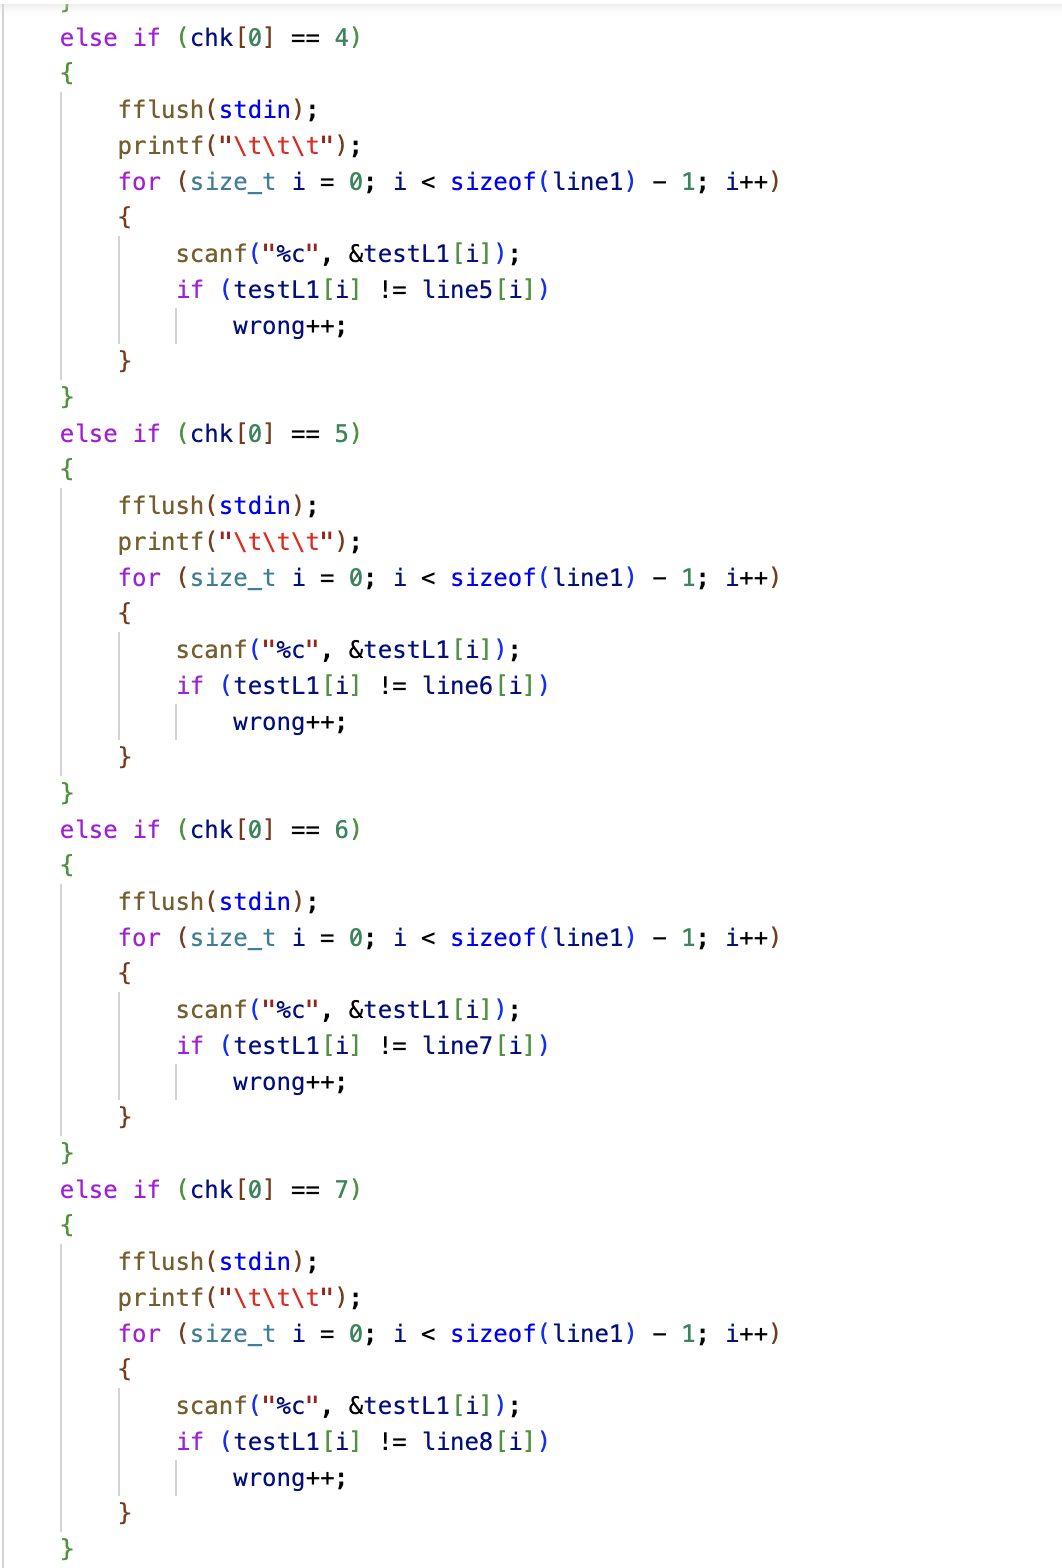
\includegraphics[scale=0.16]{CodeScreenShot/6b.png}
    \caption{Code}
    \label{fig:code-screenshots}
\end{figure}
\begin{figure}[h]
     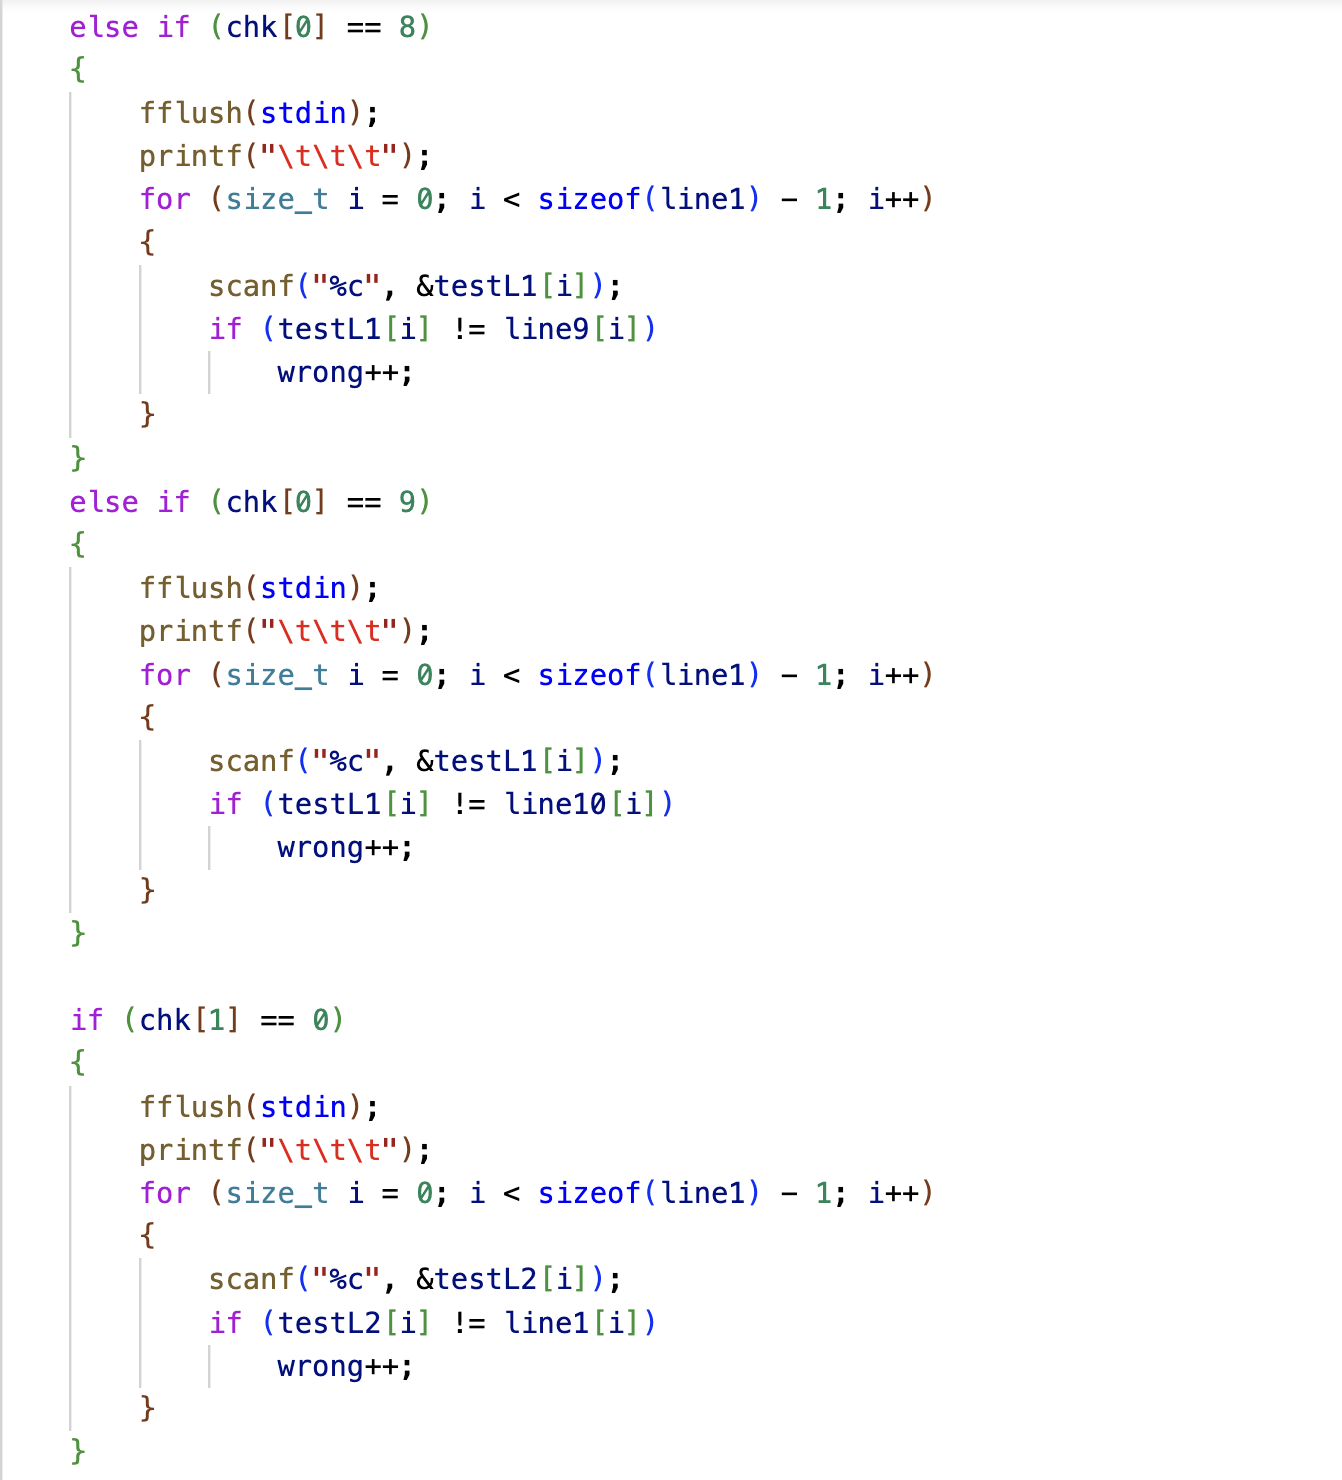
\includegraphics[scale=0.15]{CodeScreenShot/speedtest-7.png}
     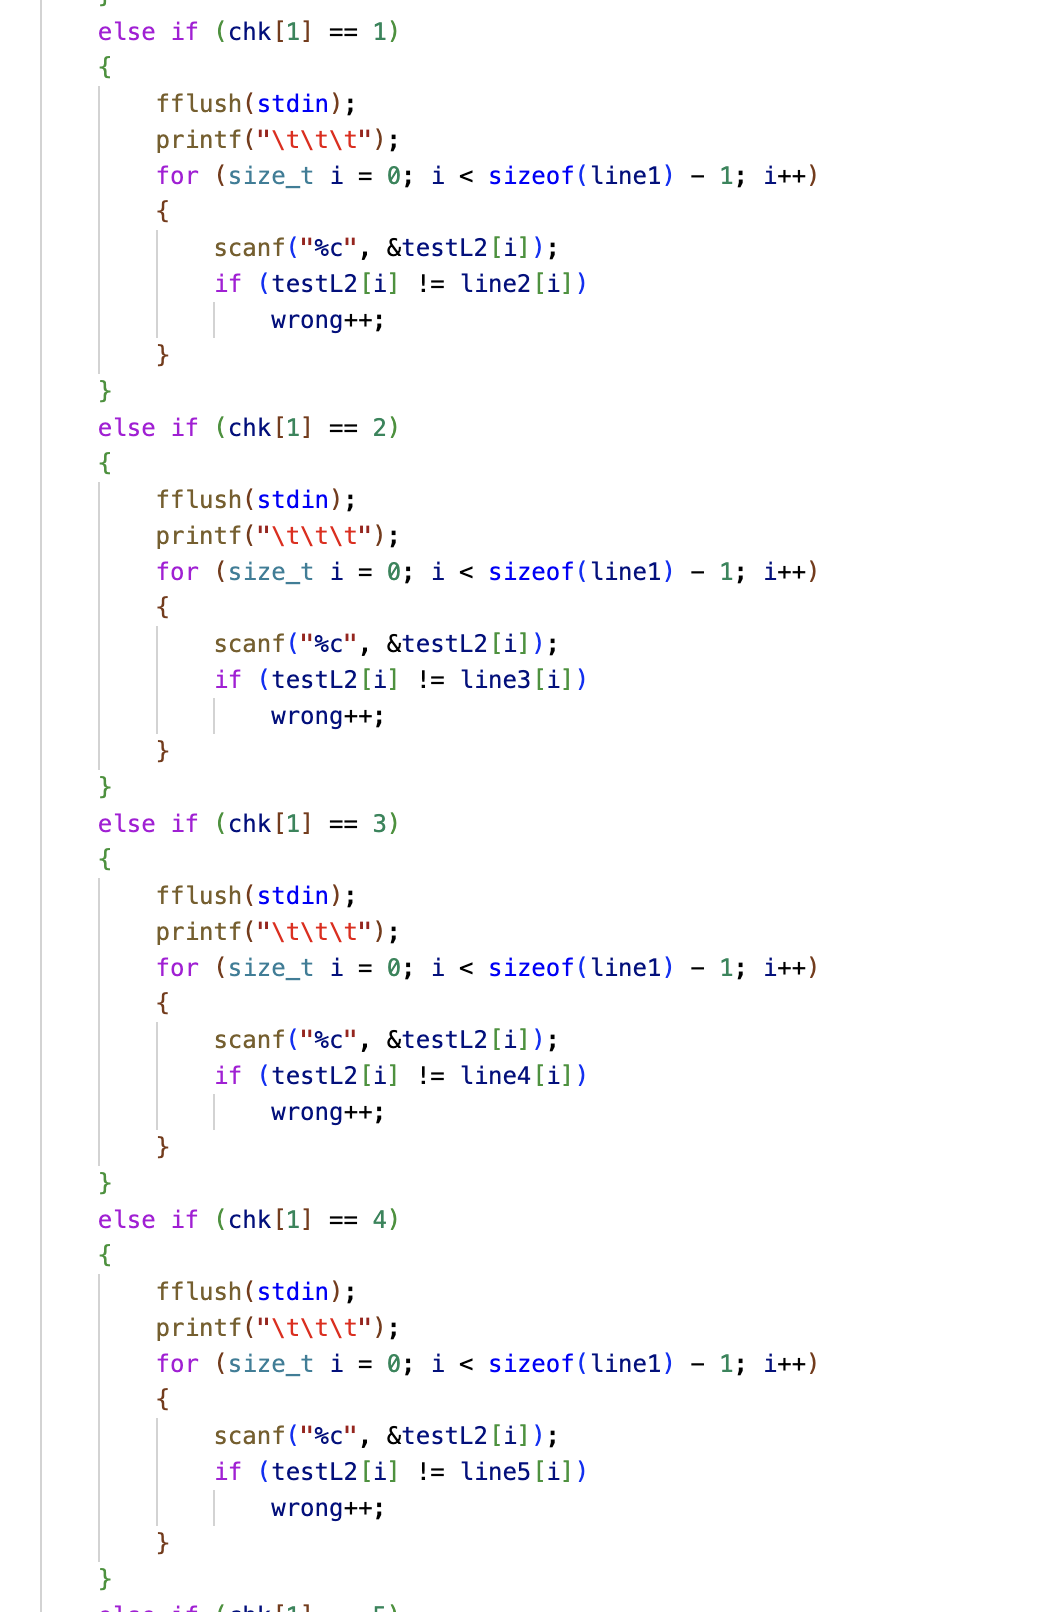
\includegraphics[scale=0.15]{CodeScreenShot/speedtest-8.png}
    \caption{Code}
    \label{fig:code-screenshots}
\end{figure}
\newpage
\begin{figure}[h]
     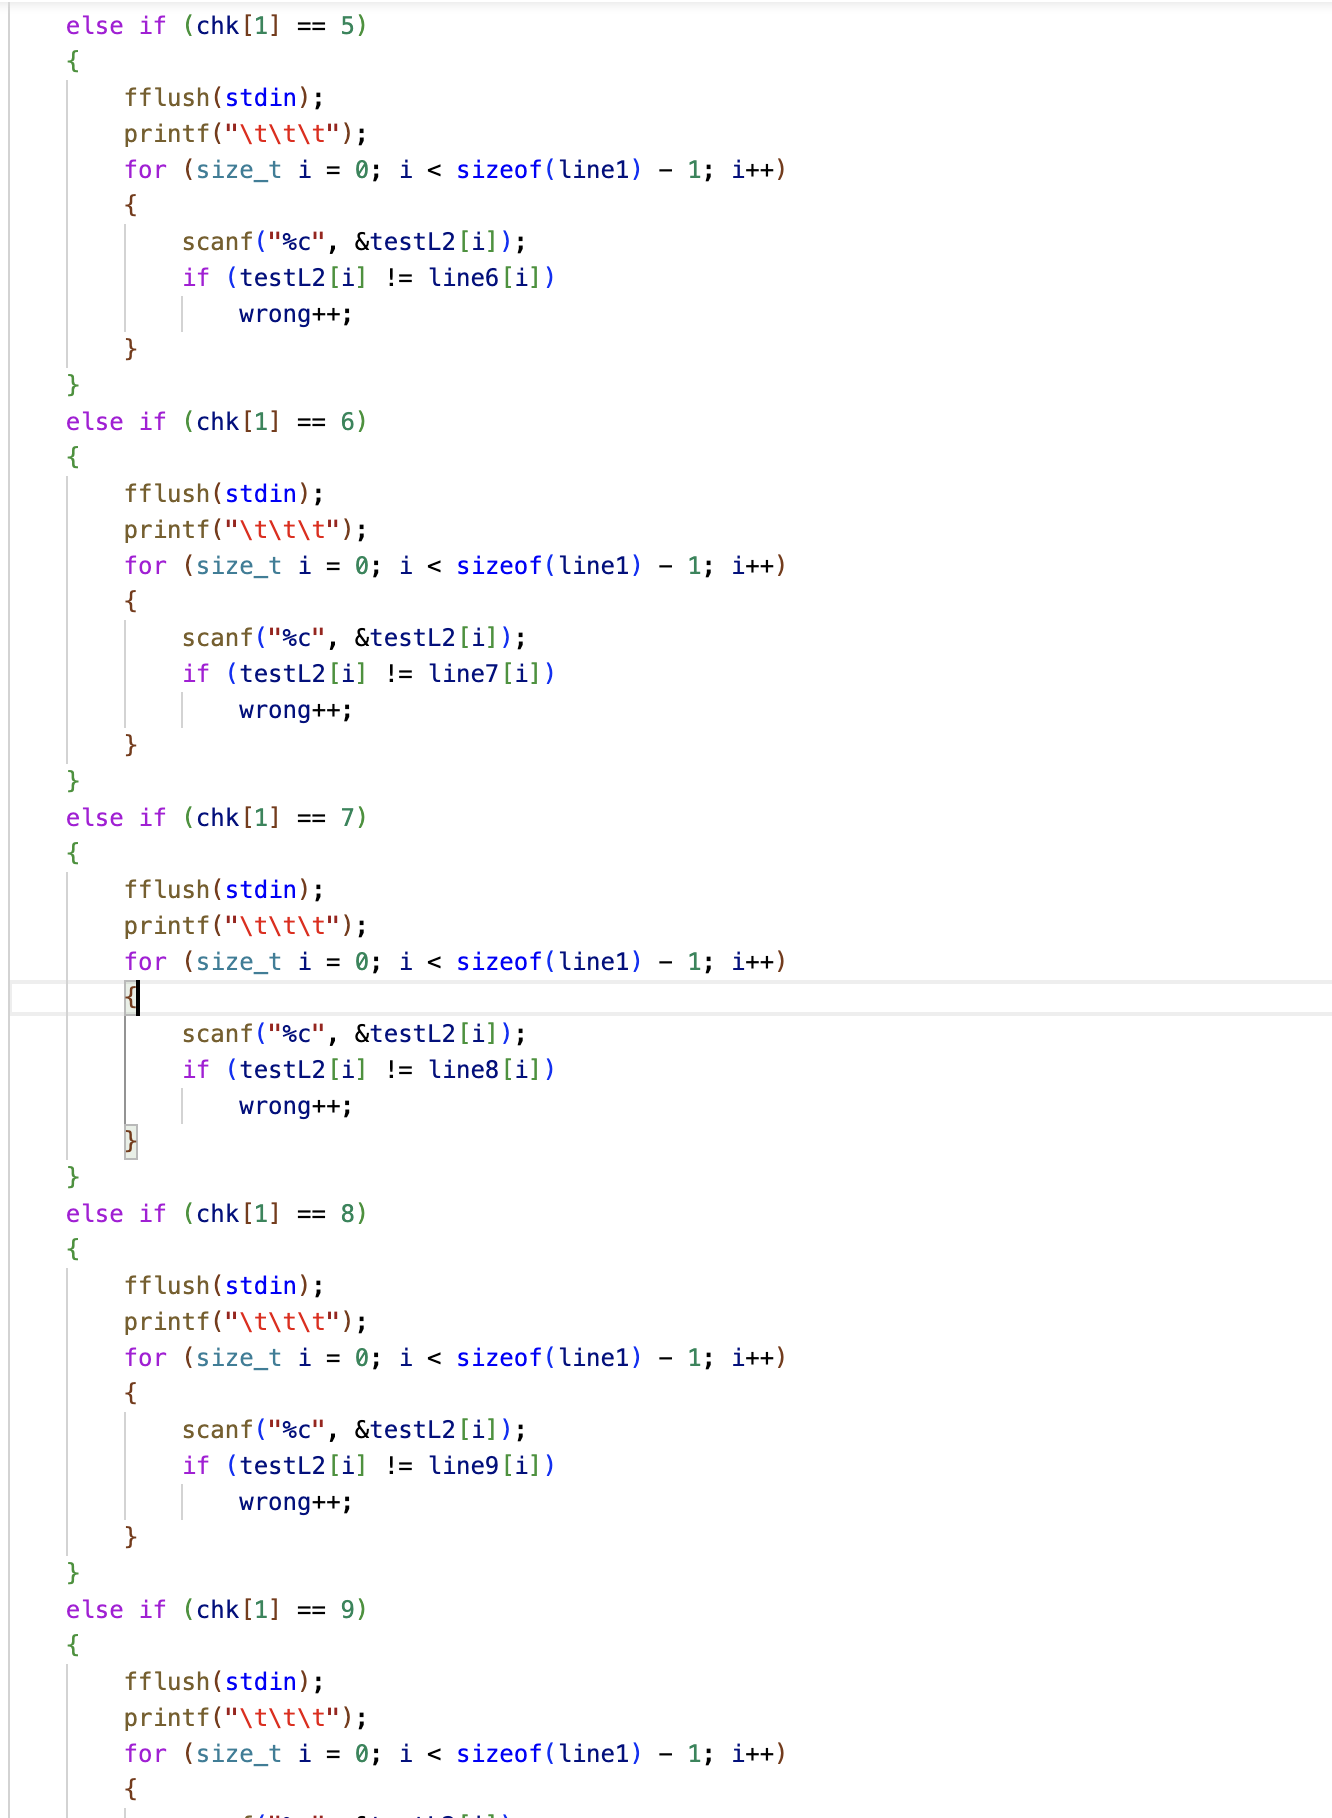
\includegraphics[scale=0.16]{CodeScreenShot/speedtest-9.png}
     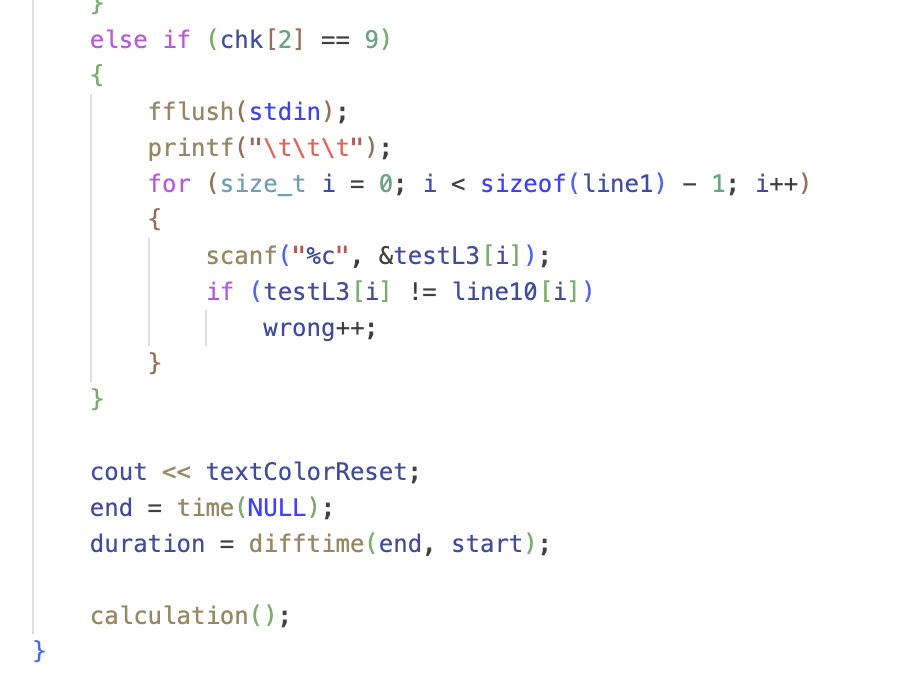
\includegraphics[scale=0.16]{CodeScreenShot/speedtest-10.png}
    \caption{Code}
    \label{fig:code-screenshots}
\end{figure}
\subsection{Programme Description}
 \begin{itemize}
        \item In this figure it is shown that the code  takes input from the user in the form of characters. The code checks the validity of the characters based on certain conditions and updates a count of 'wrong' characters if any conditions are not met.
\end{itemize}



\newpage
\begin{figure}[h]
     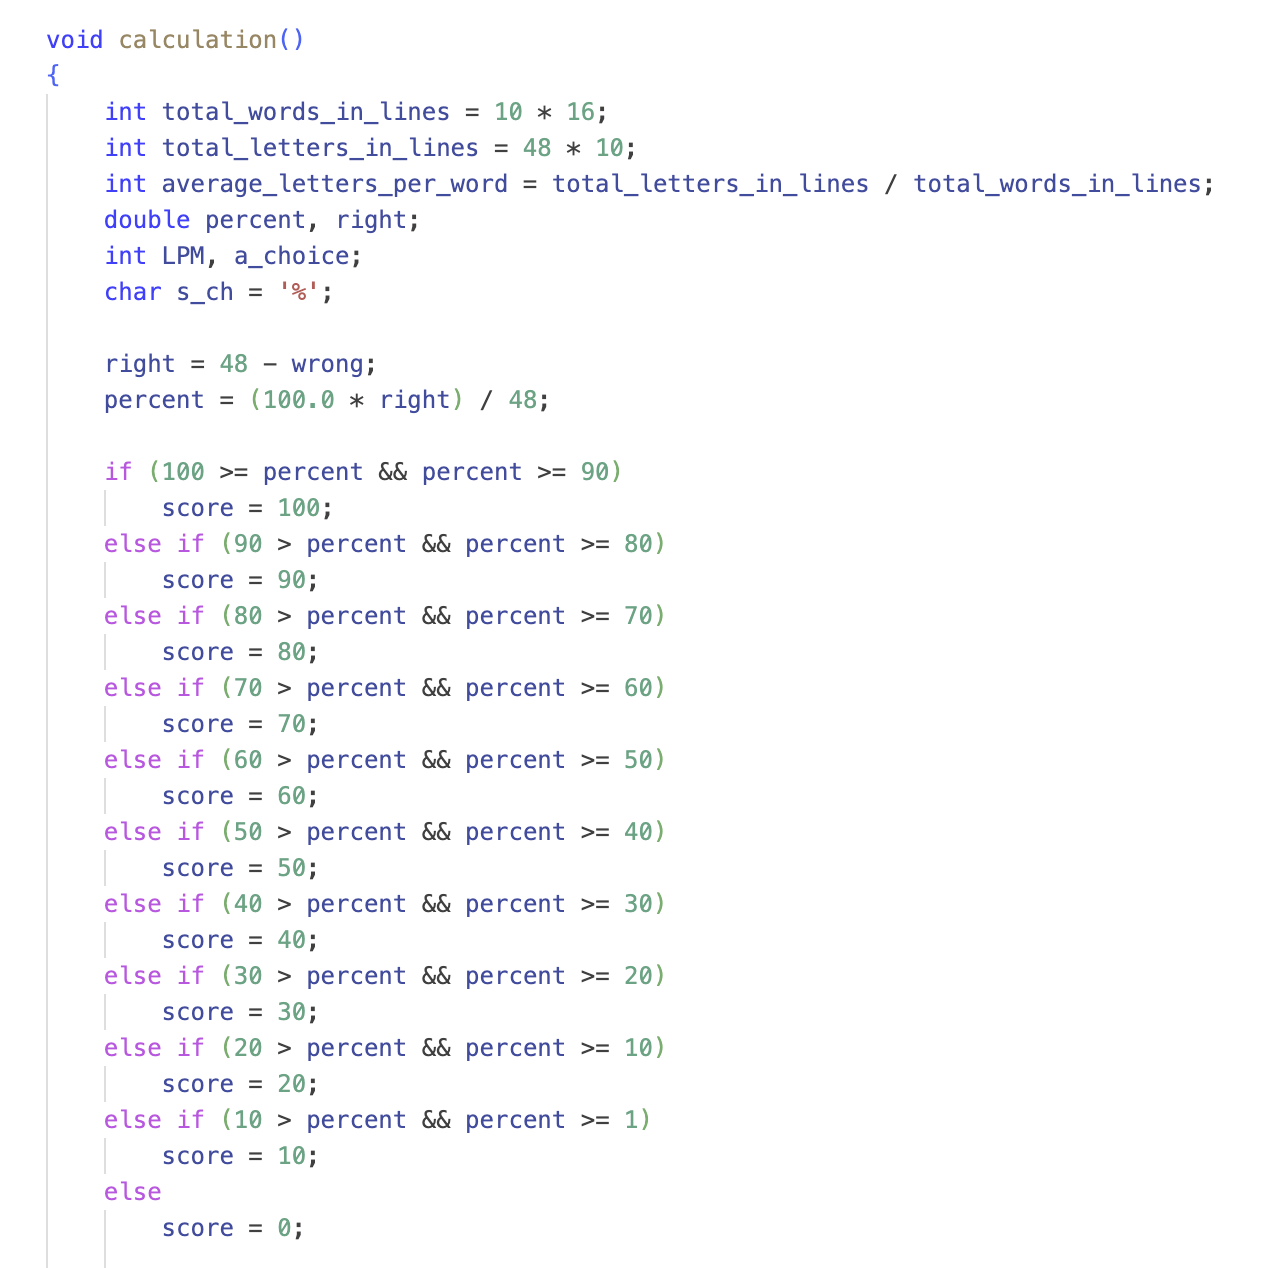
\includegraphics[scale=0.20]{CodeScreenShot/calcu-1.png}
     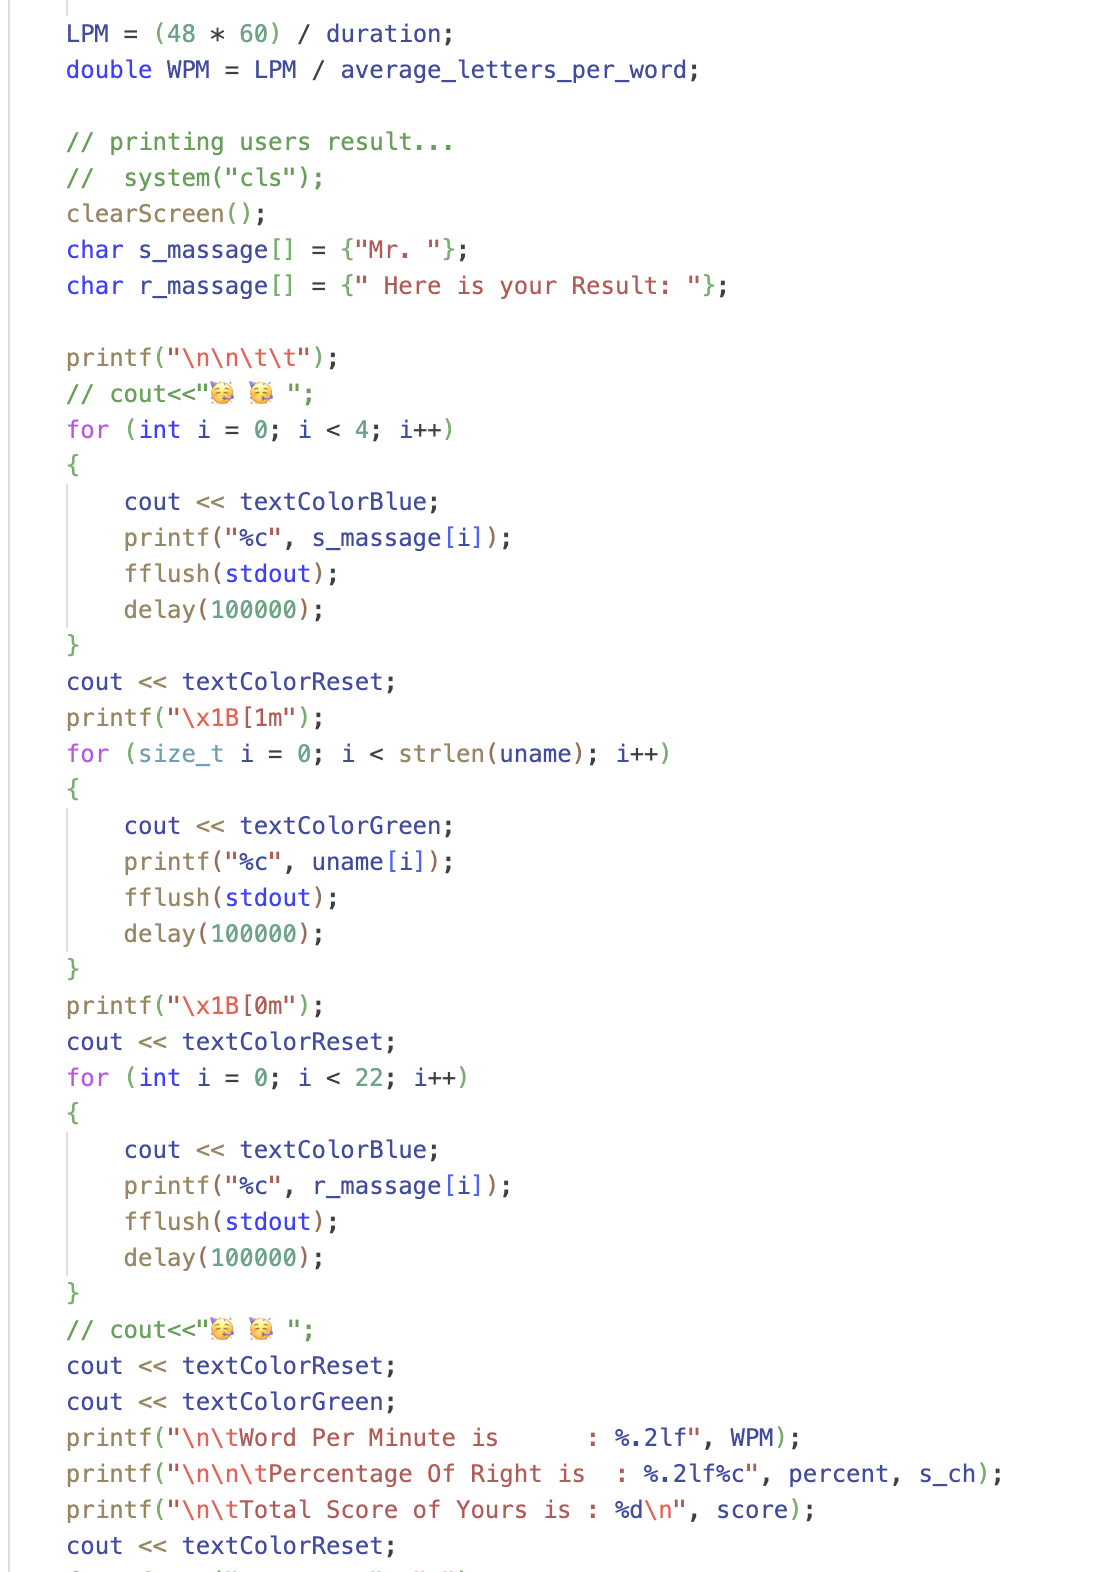
\includegraphics[scale=0.20]{CodeScreenShot/calcu-2.png}
    \caption{Code}
    \label{fig:code-screenshots}
\end{figure}

\subsection{Programme Description}

    \begin{itemize}
        \item This function, named calculation, computes various performance metrics for the user's typing test. It calculates the user's accuracy percentage, assigns a score based on the percentage achieved, and determines the Words Per Minute (WPM) and Letters Per Minute (LPM) typing speeds. The results are then presented in a visually appealing format, including a personalized message addressing the user by name and displaying the achieved WPM, accuracy percentage, and overall score. Visual effects using different text colors are employed for an enhanced user interface.
    \end{itemize}
\newpage
\begin{figure}[h]
     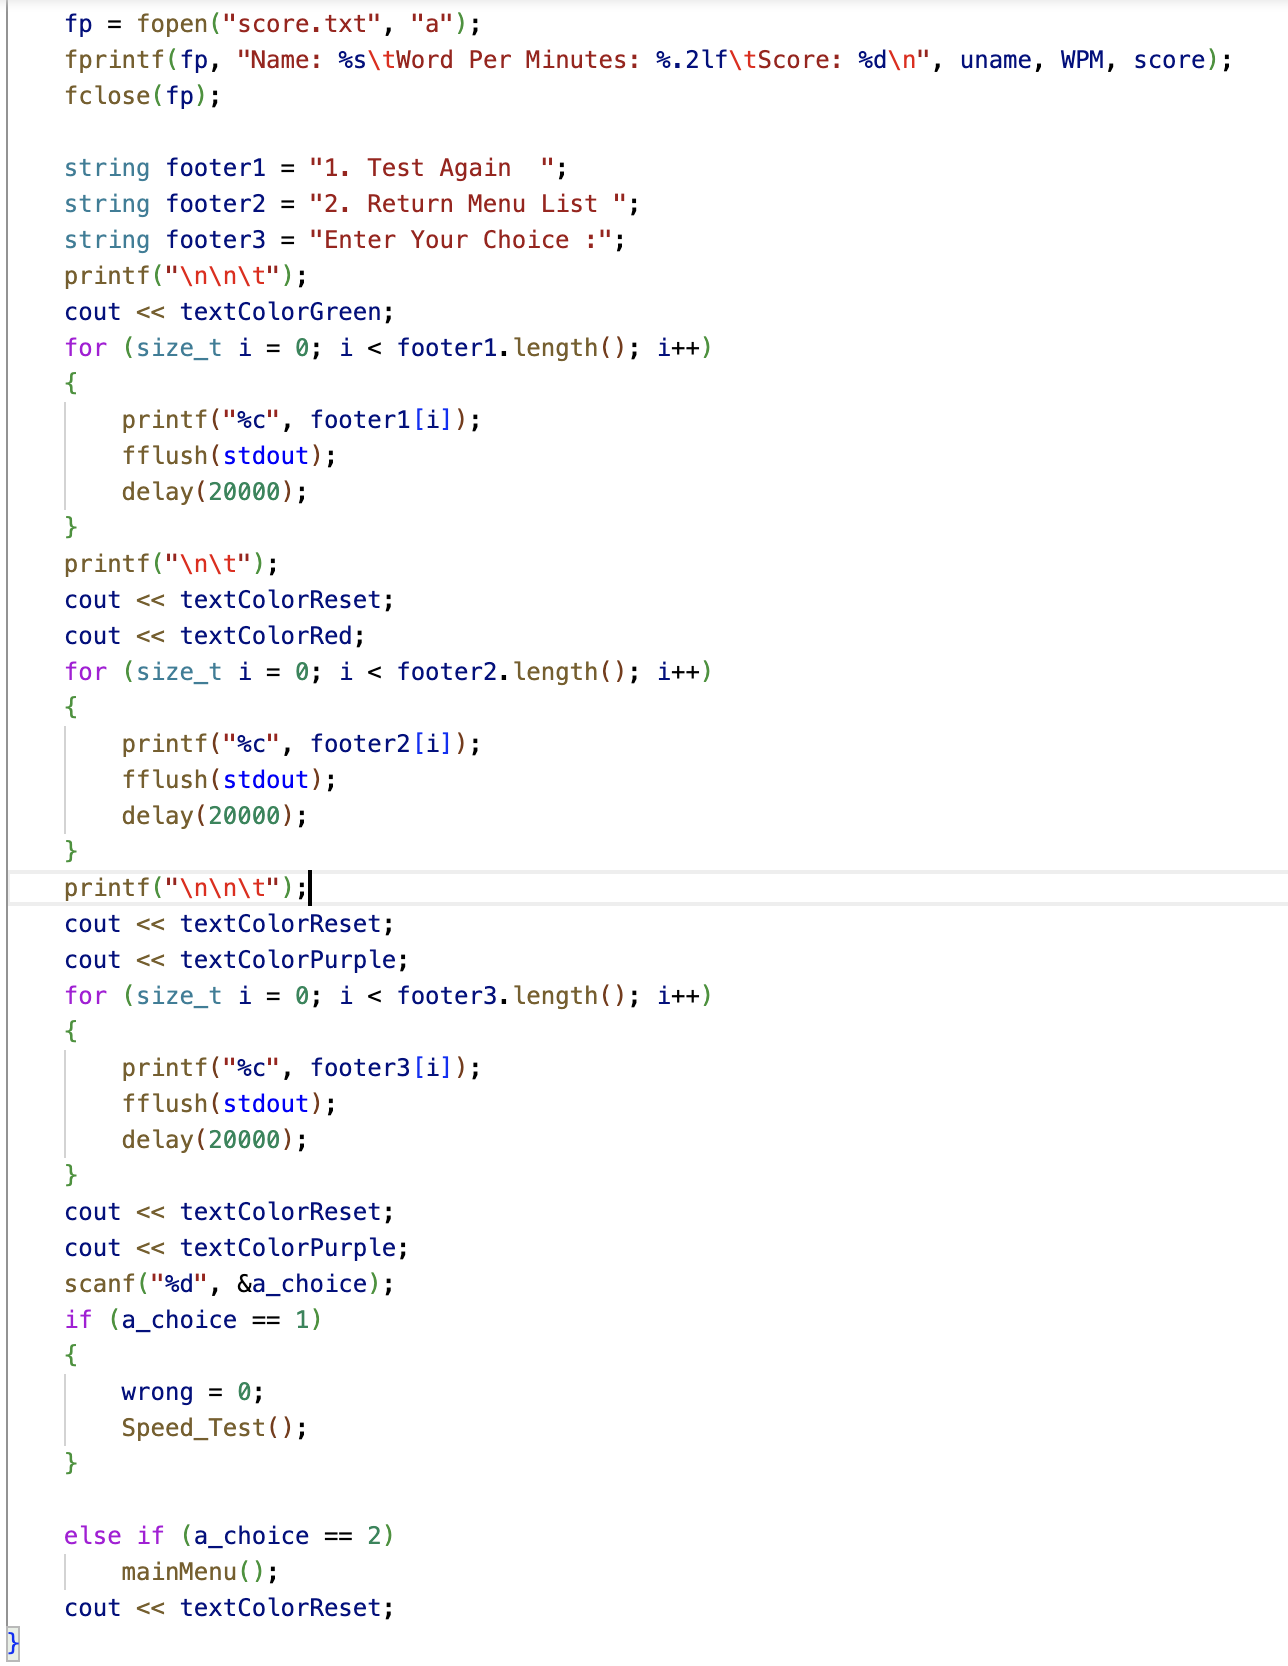
\includegraphics[scale=0.20]{CodeScreenShot/calcu-3.png}
    \caption{Code}
    \label{fig:code-screenshots}
\end{figure}

\subsection{Programme Description}
    \begin{itemize}
        \item This code snippet appends the user's performance details, including name, Words Per Minute (WPM), and score, to a file named "score.txt". It then displays a menu with options to either take the test again or return to the main menu. The user's choice is captured, and if they choose to test again, the typing test function (Speed\_Test()) is called with the wrong count reset. If they choose to return to the main menu, the main menu function (mainMenu()) is invoked. The user interface is enhanced with different text colors for a more engaging experience.
    \end{itemize}
\newpage
\begin{figure}[h]
     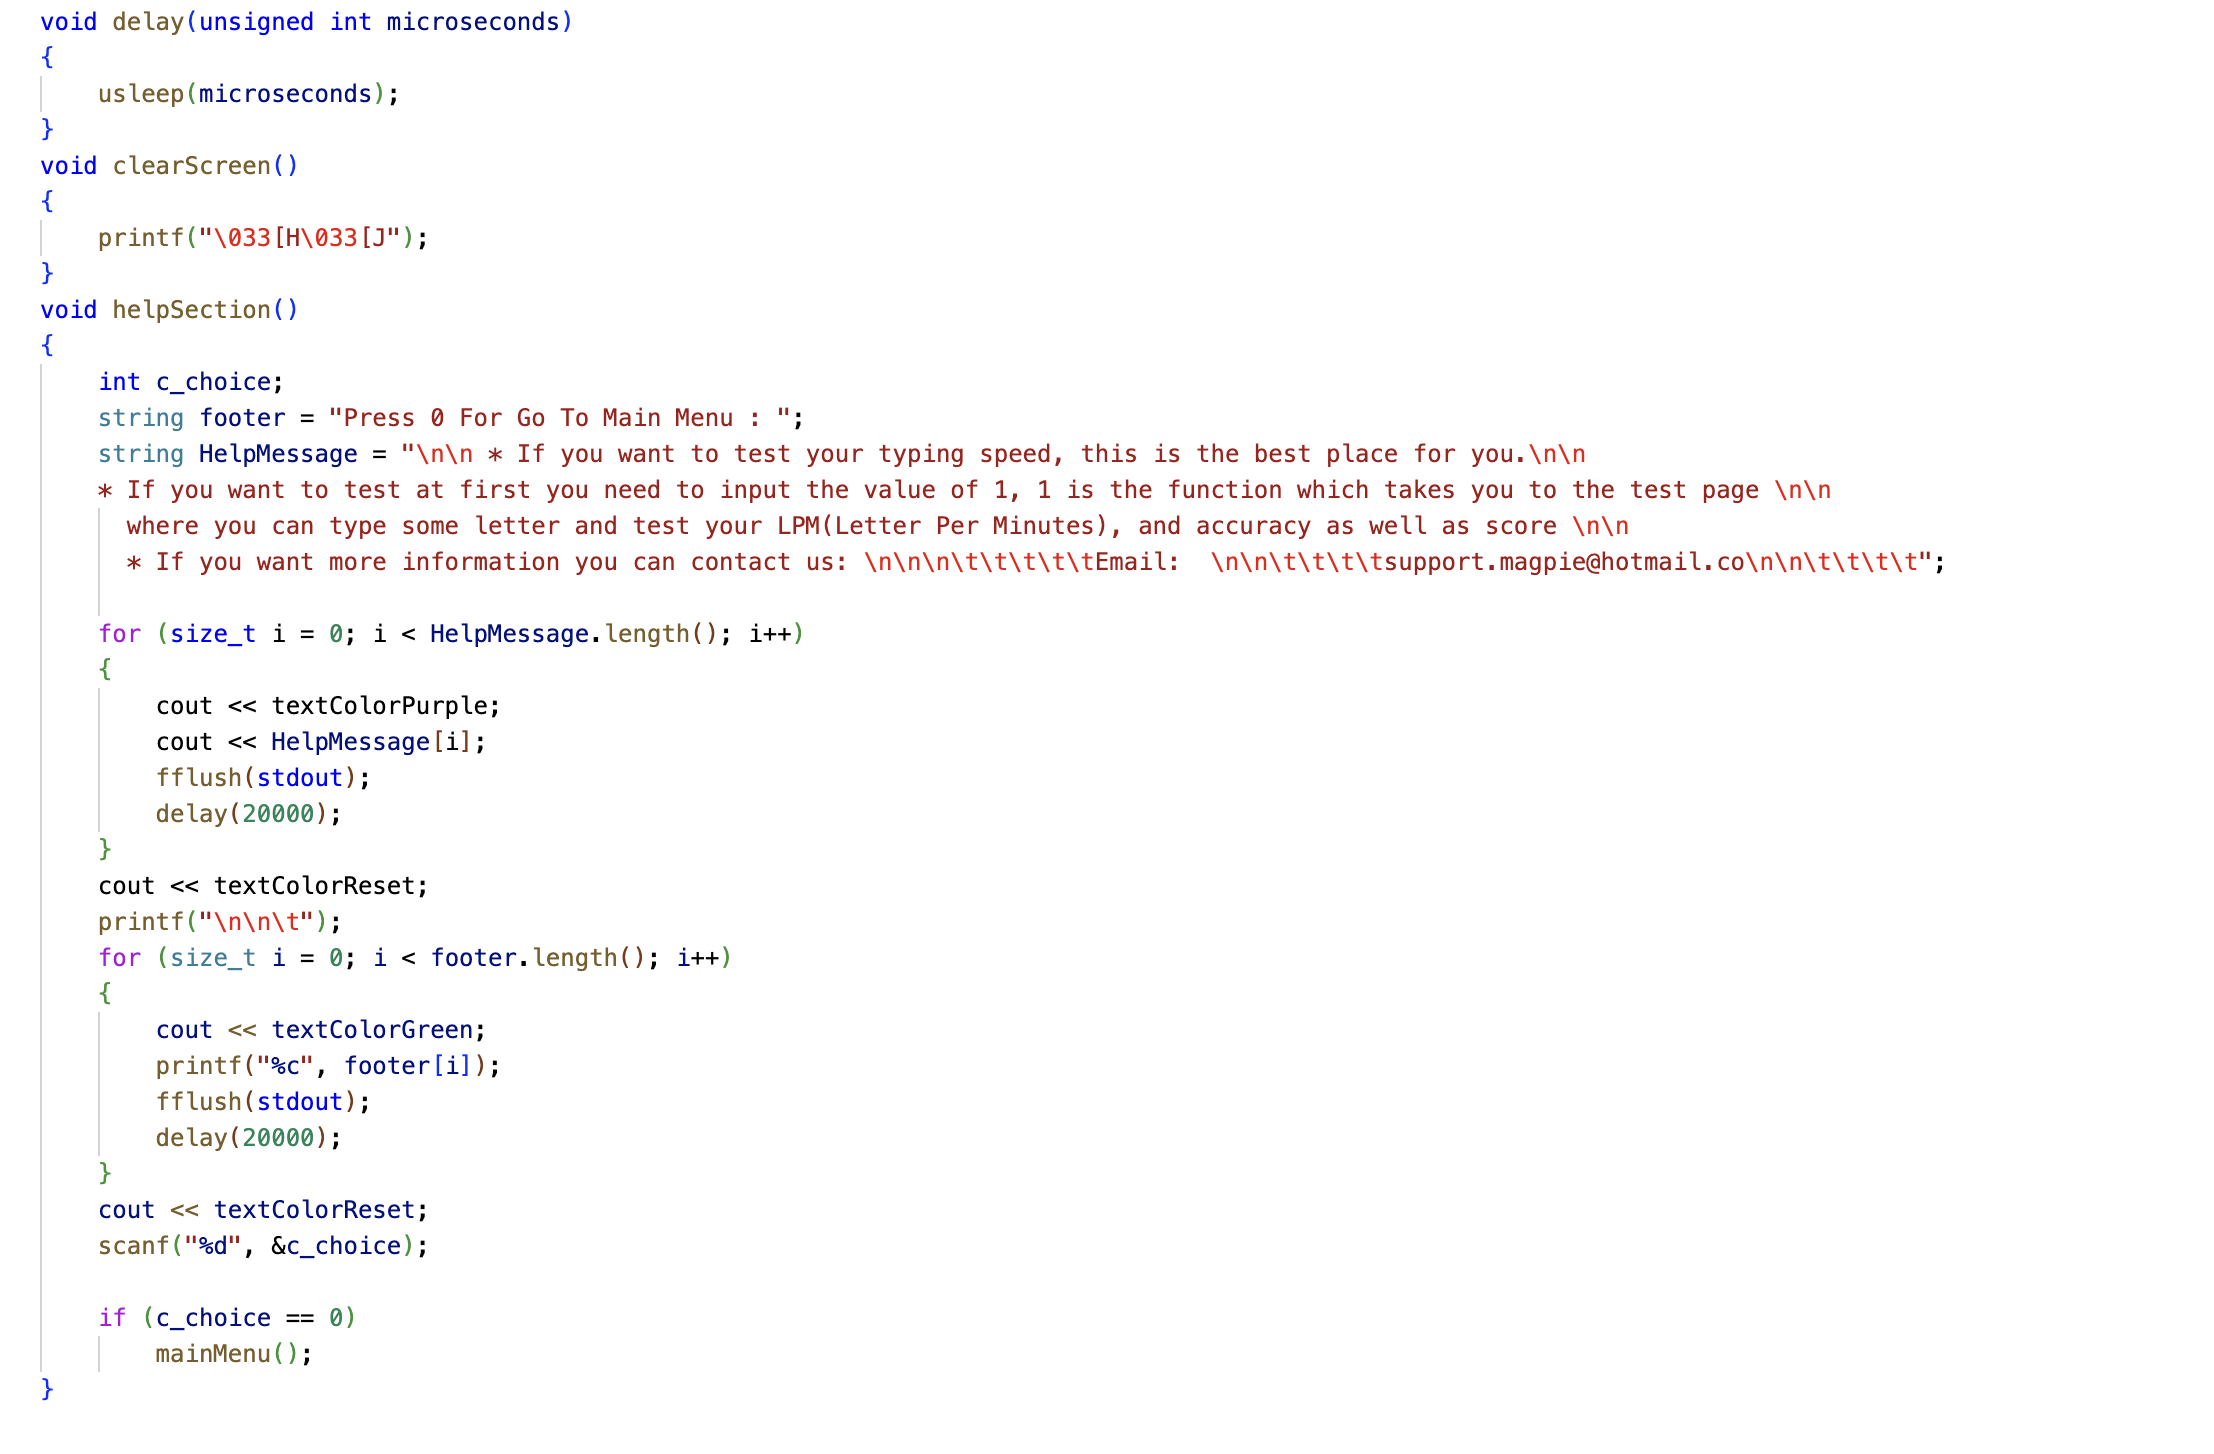
\includegraphics[scale=0.25]{CodeScreenShot/help-1.png}
    \caption{Code}
    \label{fig:code-screenshots}
\end{figure}

\subsection{Programme Description}
    \begin{itemize}
        \item This code defines three functions: delay, clearScreen, and helpSection. The delay function introduces a pause in the program for a specified duration using the usleep function. The clearScreen function is responsible for clearing the console screen. The helpSection function provides information about the typing speed testing program, including instructions on how to test typing speed. It displays a help message with contact information and prompts the user to press 0 to return to the main menu. Upon user input, it either returns to the main menu or continues with the selected option. The text is displayed with colorful formatting for an enhanced user interface.
    \end{itemize}
\newpage


\subsection{Project Output:}

\begin{figure}[h]
     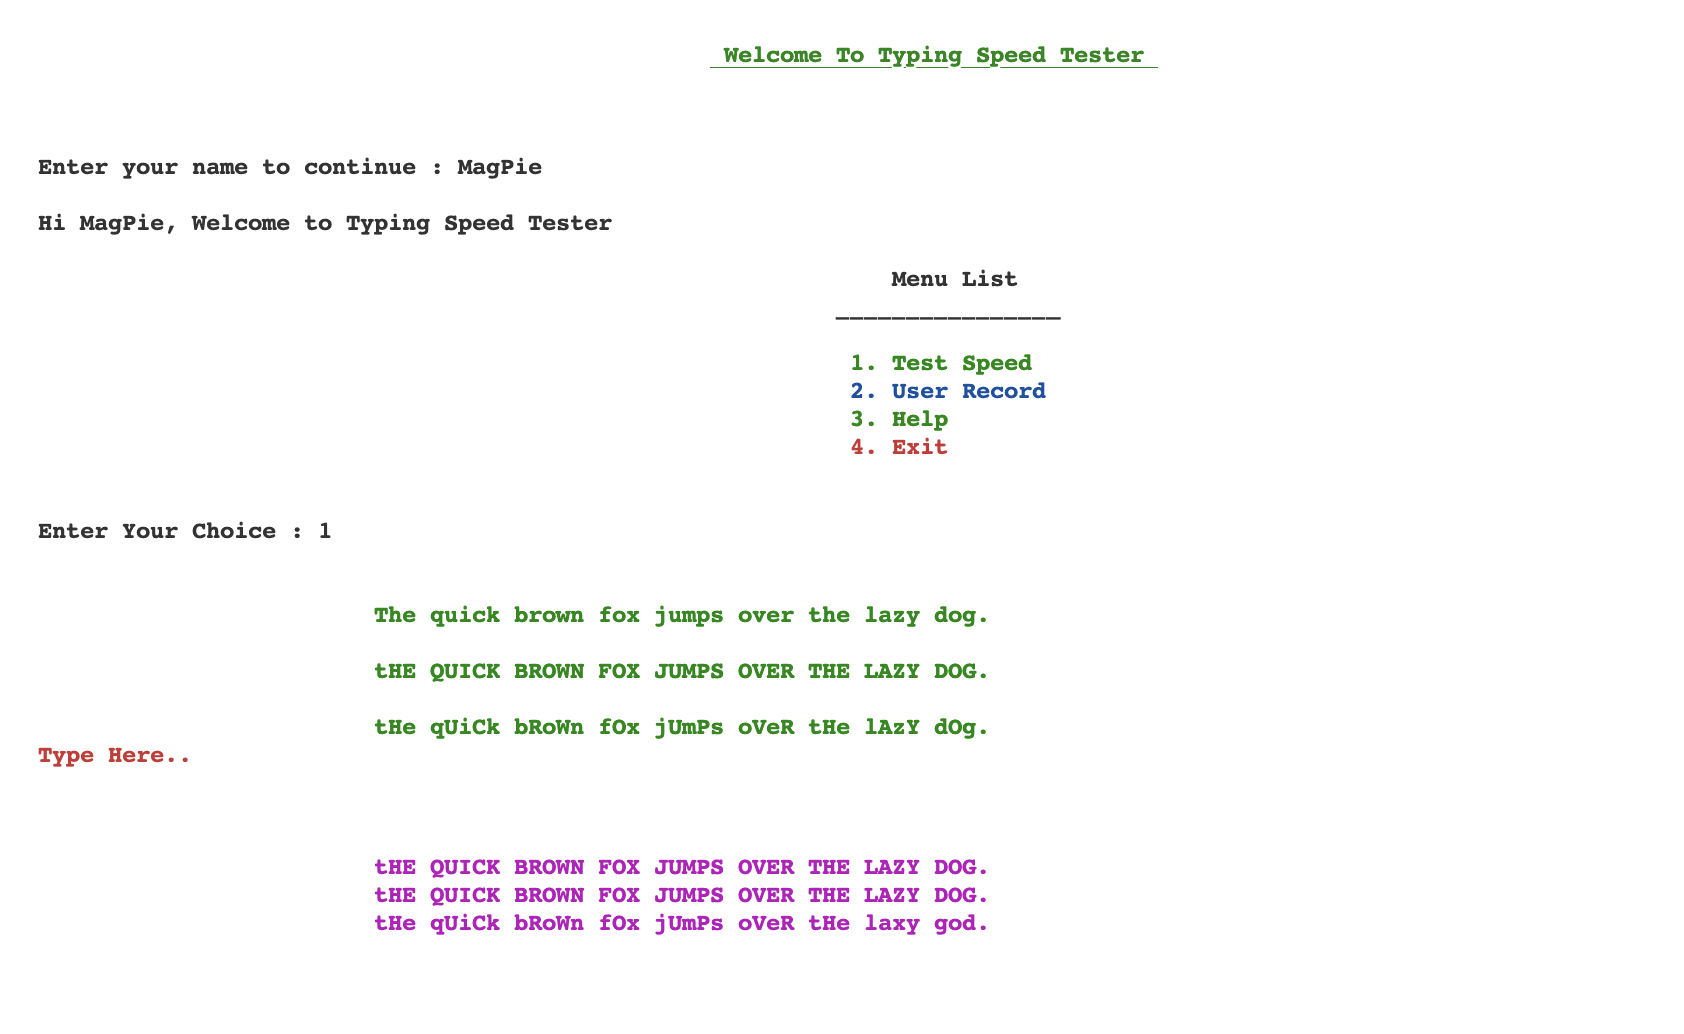
\includegraphics[scale=1,width=\textwidth]{CodeScreenShot/MagPie1.png}
    \caption{Speed Test Interface}
    \label{fig:code-screenshots}
\end{figure}
\begin{figure}[h]
     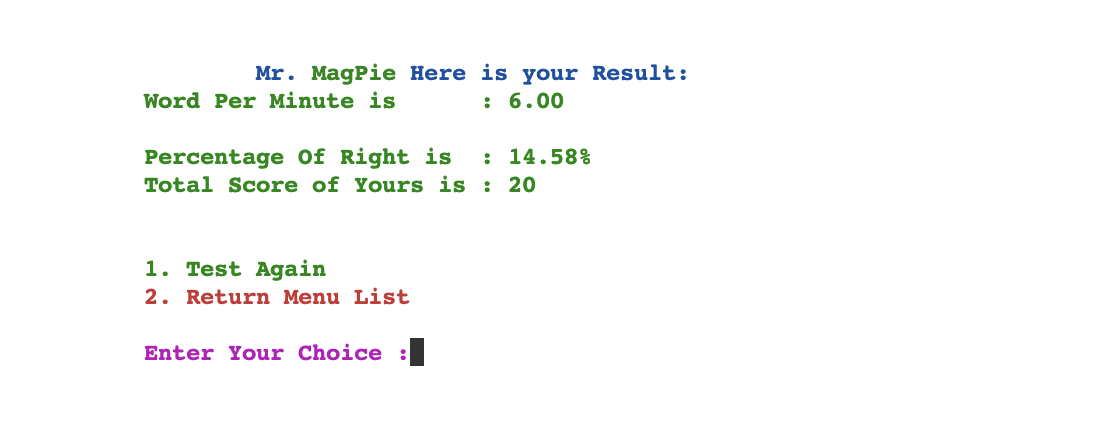
\includegraphics[scale=1,width=\textwidth]{CodeScreenShot/MagPie2.png}
    % \caption{Code}
    \label{fig:code-screenshots}
\end{figure}
\begin{figure}[h]
     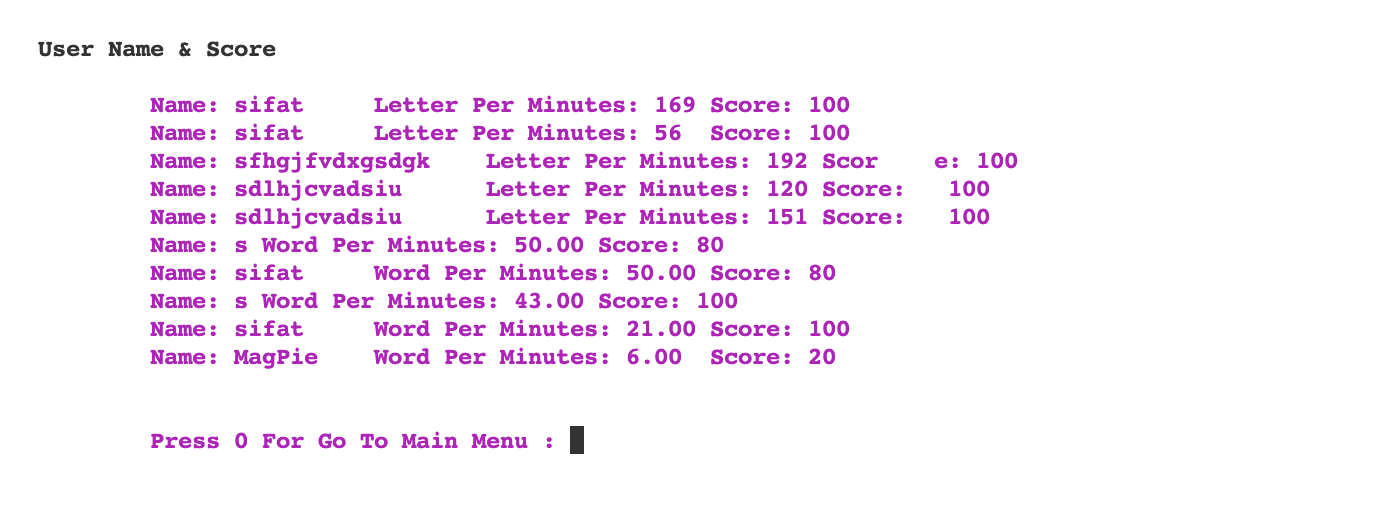
\includegraphics[scale=1,width=\textwidth]{CodeScreenShot/UserRecord.png}
    \caption{The Test Result}
    \label{fig:code-screenshots}
\end{figure}
\newpage
\begin{figure}[h]
     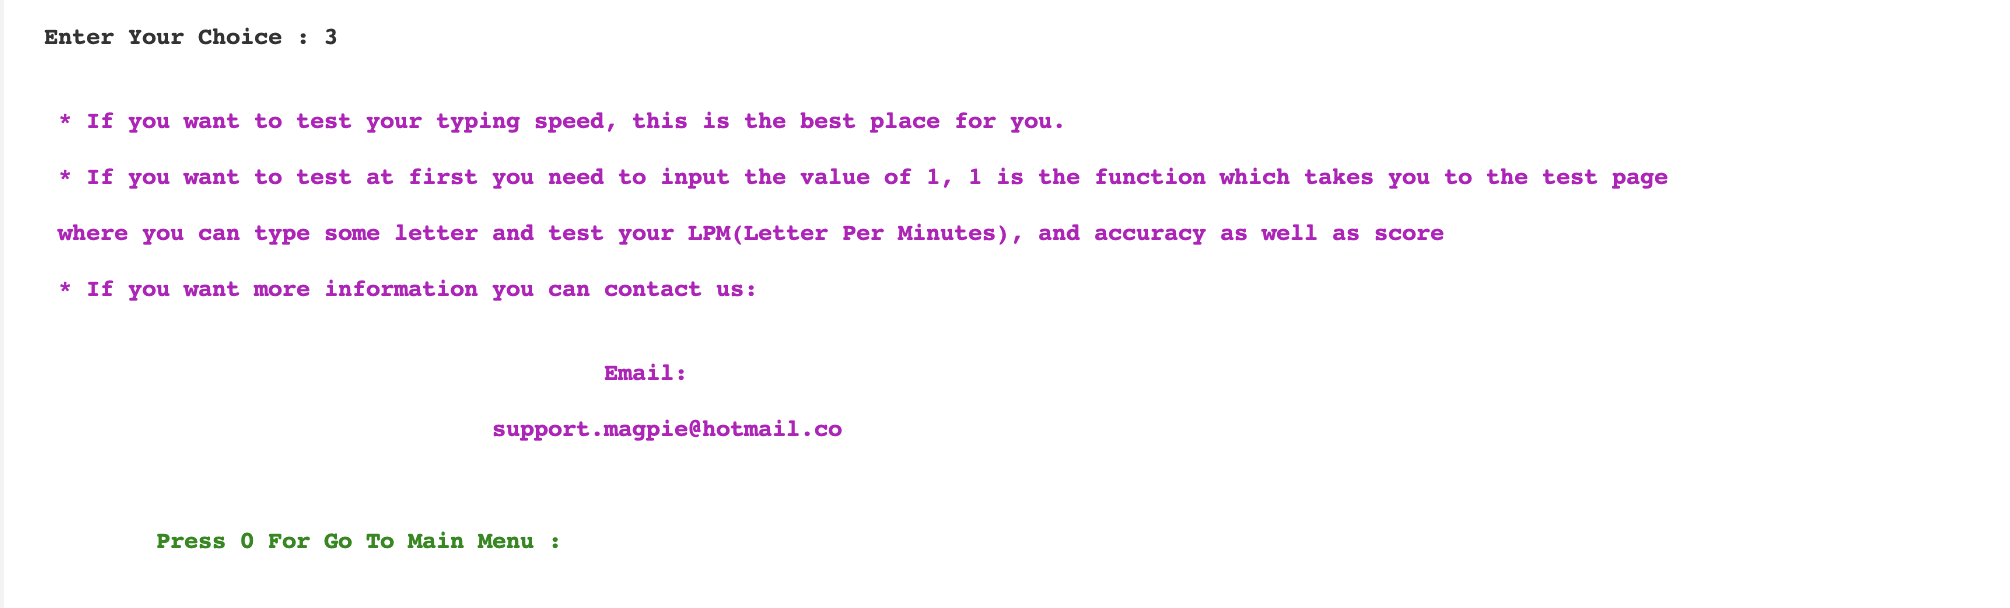
\includegraphics[scale=1,width=\textwidth]{CodeScreenShot/HelpSection.png}
    \caption{Users Previous Records}
    \label{fig:code-screenshots}
\end{figure}
\begin{figure}[h]
\centering
     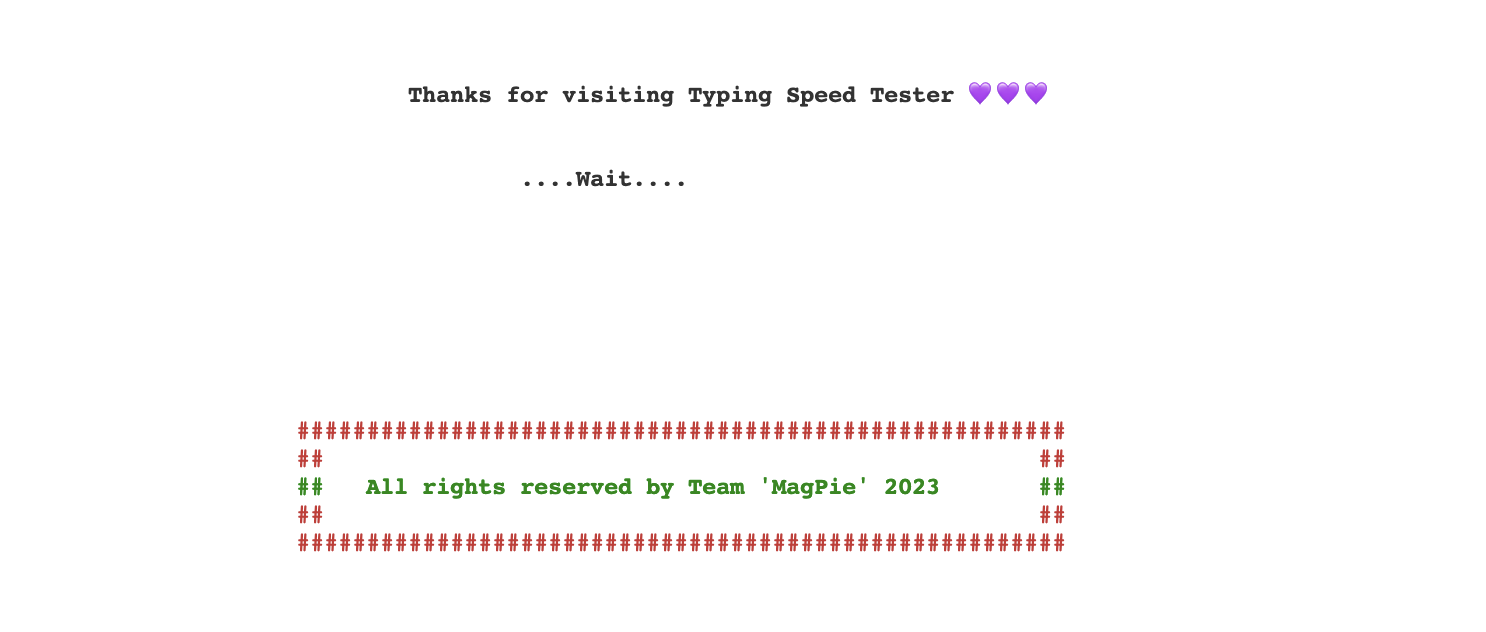
\includegraphics[scale=0.2, width={300px}]{CodeScreenShot/Ending line.png}
    \caption{Greetings}
    \label{fig:code-screenshots}
\end{figure}
\newpage

\subsection{Feasibility analysis}

\begin{itemize}
    \item \textbf{Technical Feasibility: } The technical feasibility of a typing speed tester project involves evaluating technology and infrastructure availability. This includes assessing compatibility with different devices and platforms, scalability, performance requirements, reliable internet connectivity, and server infrastructure. Security measures, such as data encryption and protection against hacking, are crucial. Overall, careful consideration of the technology stack, infrastructure, and security measures ensures a smooth and reliable user experience.


\item \textbf{Economic Feasibility: }The Economic Feasibility of the Typing Speed Tester project underscores its cost-effectiveness and financial sustainability. Leveraging open-source tools minimizes software acquisition costs, while the project's efficient design reduces hardware requirements. Scalability ensures optimal performance under varying user loads without substantial infrastructure investment. With low maintenance needs, the project promises long-term cost savings. In summary, the Typing Speed Test project presents an economically feasible solution, providing value with minimal upfront, operational, and maintenance expenses.

\item \textbf{Operational Feasibility: }The Operational Feasibility of the Typing Speed Tester project is characterized by its user-friendly interface, minimal training requirements, and efficient data management. The system seamlessly integrates into user workflows, ensuring ease of adoption and smooth administration. With scalability to accommodate diverse user levels, the project is operationally robust, aligning effectively with user needs and streamlining administrative processes. Overall, its operational feasibility is a key strength, contributing to the project's success and user satisfaction.
\par

\item \textbf{Schedule Feasibility: }The Schedule Feasibility of the Typing Speed Tester project demonstrates a well-structured and realistic timeline for development, testing, and implementation. The project adheres to predefined milestones, allowing for efficient task management and timely delivery. Regular progress assessments and flexible adjustments ensure adaptability to unforeseen challenges, enhancing the project's overall schedule feasibility. The project's timeline aligns with the outlined goals, reflecting a commitment to on-time completion and successful integration into the designated timeframe.
\end{itemize}
\subsection{Requirement Analysis}
 Typing Speed Tester project involves a thorough examination of functional and non-functional specifications. Functionally, the system must accurately measure typing speed and assess accuracy based on provided paragraphs. User authentication and result storage are essential. Non-functional requirements include a user-friendly interface, cross-platform compatibility, and efficient processing to ensure real-time feedback. Accessibility features for differently-abled users should also be considered. Additionally, scalability to accommodate future enhancements and security measures to protect user data are integral aspects of the project's requirement analysis. The analysis forms the foundation for the successful development and implementation of the Typing Speed Test project.


\subsection{The Project Methodology}
The project methodology for the Typing Speed Tester involves a systematic approach to ensure effective development and implementation. The methodology can be outlined as follows:

\begin{enumerate}
    \item  Project Planning:Define project scope, objectives, and deliverables. Develop a detailed project plan outlining tasks, timelines, and resource allocation.

\item  Requirement Analysis: Conduct a thorough analysis of functional and non-functional requirements. Identify key features, user interactions, and system constraints.

\item  Design:Create a detailed system design, including the user interface, backend logic, and database structure. Ensure scalability, responsiveness, and a user-friendly experience.

\item  Implementation: Code the application using C++ programming language. Implement features such as user input processing, speed calculation, accuracy assessment, and result display.

\item  Testing: Conduct extensive testing, including unit testing, integration testing, and user acceptance testing. Ensure the system functions accurately and meets all specified requirements.

\item Documentation: Create comprehensive documentation, including user manuals and technical documentation. This aids in system maintenance and user guidance.

\item  Deployment: Deploy the Typing Speed Test application on suitable platforms. Ensure compatibility and performance in different environments.

\item User Training: Provide training materials or sessions for users to understand how to use the Typing Speed Test effectively.

\item Feedback and Iteration: Collect user feedback and make iterative improvements to enhance the application's performance, usability, and features.
\vspace{6px}
By following this methodology, the Typing Speed Test project can be systematically developed, ensuring a robust and user-friendly application.
\end{enumerate}

\subsection{Data Collection \& Prepossessing }

\textbf{Data Collection}
\begin{enumerate}
    \item User Input: Capture the user's input as they type the provided text. This includes recording the characters typed, the time taken to type each character, and any errors made.

\item Device Information: Collect information about the user's device, such as their keyboard type, browser version, and operating system. This information can be used to contextualize the typing performance data.

\item User Demographics: Optionally, collect demographic information about the user, such as their age, location, and occupation. This information can be used to analyze typing speed trends across different demographics.
\end{enumerate}
\newpage

\textbf{Data Processing}

\begin{enumerate}
    \item Cleaning and Preprocessing: Clean the collected data to remove any inconsistencies or errors. This may involve handling typos, removing illegal characters, and normalizing timestamps.

\item  Feature Extraction: Extract relevant features from the data. These features may include:
   - Typing Speed: Calculate the average typing speed in words per minute (WPM) and characters per minute (CPM).
   - Accuracy: Calculate the percentage of characters typed correctly.
   - Error Analysis: Identify common errors made by the user, such as typos, missed characters, and extra characters.

\item  Performance Analysis: Analyze the typing speed and accuracy data to identify patterns and trends. This may involve comparing performance across different text types, user demographics, and device types.

\item  Data Visualization:Create visualizations to represent the analyzed data, such as charts, graphs, and tables. These visualizations can be used to communicate insights to users and stakeholders.

\item Data Storage:Store the collected and processed data in a secure and accessible manner. This may involve using a database or a cloud storage service.
\end{enumerate}
\subsection{Algorithm}
The Speed Typing Tester project involves several algorithms to achieve its functionalities. Here is an overview of the key algorithms implemented in the code:

\begin{enumerate}
    \item \textbf{Typing Speed Calculation Algorithm:
}   Randomly selects three paragraphs for the user to type.
   - Measures the time taken by the user to complete typing.
   - Calculates the typing speed in Letters Per Minute (LPM) and Word Per Minute (WPM).
   - Evaluates the accuracy of the user's input.

\item \textbf{ Scoring Algorithm:
}    Computes the percentage of correctly typed characters.
   Assigns a score based on the percentage achieved.
    Utilizes a grading system to categorize users into different proficiency levels.

\item\textbf{File Handling Algorithm:
}    Manages user records by reading and writing to a file .
    Appends new records for each typing test, including the user's name, LPM, and score.

\item\textbf{User Interface Animation Algorithm:
}    Utilizes ANSI escape codes for colorful and dynamic console output.
   Delays output to create a typewriter-like effect, enhancing user engagement.
    Clears the console screen for a clean and organized interface.

\item\textbf{Menu Navigation Algorithm:
} Implements a menu-driven interface for user interaction.
   Allows users to choose between typing tests, viewing records, accessing help, and exiting the program.
    Facilitates navigation between different sections of the program.

\item\textbf{Help Section Algorithm:
}    Displays information about the purpose and usage of the typing speed tester.
    Provides contact details for support.

\item\textbf{Delay and Clear Screen Algorithm:
}   Implements delay functions to control the speed of text output, creating a smooth and visually appealing display.
    Clears the console screen for better readability and an organized interface.

\end{enumerate}



\subsection{Design and Implementation}
The  Speed Typing Tester project reflect a structured and user-friendly approach. The code is organized into modular functions for distinct functionalities. The project follows a console-based interface, engaging users with colorful and dynamic elements. The implementation employs features like file handling for user records and time functions for speed calculations. The code structure is well-commented, promoting readability and easy maintenance. The design incorporates a welcoming interface, and the code adheres to good programming practices, enhancing its effectiveness as a typing speed assessment tool. Overall, the project seamlessly integrates functionality with a visually appealing design for an interactive user experience.






\subsection{Results and Discussion}

The Typing Speed Tester project achieves accurate assessments and fosters user improvement through effective algorithms. Its user-friendly interface and scalability enhance the experience, while a comprehensive dataset enables diverse evaluations. Discussions in the Results and Discussion section underscore the project's potential to enhance typing skills, making it a valuable tool for skill development.

